%% Paper 1. Layout follows the AGU journal class used by van Leeuwen (arXiv:2601.01795):
%% PJ2019.cls (= AGU agujournal2019.cls, 2019-04-16), `draft` option, apacite author-year
%% citations. The REVTeX/Chaos version of 2026-10-08 is superseded by this one.
\PassOptionsToPackage{natbibapa}{apacite}% keep \citet / \citep with apacite
\documentclass[draft]{PJ2019}

\usepackage{amsmath,amssymb}
\usepackage{amsthm}
\usepackage{mathtools}
\usepackage{bm}
\usepackage{booktabs}
\usepackage{xcolor}
\usepackage{xspace}
\usepackage[group-separator={,}]{siunitx}
\usepackage[hidelinks]{hyperref}

% Shared notation for paper 1.
\newcommand{\DKY}{D_{\mathrm{KY}}}
\newcommand{\dlat}{d_{\mathrm{lat}}}
\newcommand{\Nens}{N_{\mathrm{ens}}}
\newcommand{\R}{\mathbb{R}}
\newcommand{\Z}{\mathbb{Z}}
\newcommand{\E}{\mathcal{E}}          % encoder
\newcommand{\Dec}{\mathcal{D}}        % decoder
\newcommand{\Fp}{\mathcal{F}}         % latent propagator
\newcommand{\Hobs}{\mathcal{H}}       % physical observation operator
\newcommand{\Lat}{\Lambda}            % site lattice
\newcommand{\Shift}{\mathsf{S}}       % lattice shift
\newcommand{\Tr}{\mathsf{T}}          % physical translation
\newcommand{\Exp}{\mathbb{E}}
\newcommand{\Var}{\operatorname{Var}}
\newcommand{\Cov}{\operatorname{Cov}}
\newcommand{\tr}{\operatorname{tr}}
\newcommand{\dist}{\operatorname{dist}}
\newcommand{\Renc}{R_{\mathrm{enc}}}
\newcommand{\Rdec}{R_{\mathrm{dec}}}
\newcommand{\Rprop}{R_{\mathrm{prop}}}
\newcommand{\kmax}{k_{\max}}
\newcommand{\kmid}{k_{\mathrm{mid}}}
\newcommand{\wvar}{w_{\mathrm{var}}}
\newcommand{\wld}{w_{\mathrm{ld}}}
\newcommand{\ie}{i.e.\@\xspace}
\newcommand{\eg}{e.g.\@\xspace}

\newtheorem{proposition}{Proposition}
\newtheorem{lemma}{Lemma}
\newtheorem{corollary}{Corollary}
\theoremstyle{remark}
\newtheorem{remark}{Remark}

% Run-in paragraph heading (revtex letters \paragraph headings; we do not want that).
\newcommand{\para}[1]{\par\medskip\noindent\textbf{#1}\enspace}

% Wide table that is scaled to the text width (revtex's ruledtabular forces \hsize and defeats
% \resizebox). Same double-rule look as ruledtabular. #1: column spec, #2: body (header + rows).
\newcommand{\widetabular}[2]{\resizebox{\textwidth}{!}{%
  \begin{tabular}{#1}\hline\hline\noalign{\vskip 2pt}#2\noalign{\vskip 2pt}\hline\hline\end{tabular}}}
% Table bodies are read with TeX's primitive \input (expandable), so a rule may follow them.
\makeatletter\newcommand{\tabinput}[1]{\@@input #1.tex }\makeatother

% REVTeX's ruledtabular (used by every table) for non-REVTeX classes: centred table with
% double rules above and below; the table body supplies its own \hline after the header.
\makeatletter
\@ifundefined{ruledtabular}{%
\newenvironment{ruledtabular}{\par\centering
  \let\rt@tabular\tabular \let\rt@endtabular\endtabular
  \renewenvironment{tabular}[1]{\rt@tabular{##1}\hline\hline\noalign{\vskip2pt}}%
    {\noalign{\vskip2pt}\hline\hline\rt@endtabular}}{\par}}{}
\makeatother

% Placeholder for numbers that pending runs will fill (Block K; see docs/paper1/partII_narrative.md,
% table P1-P12). Renders in red so none survives into a submitted draft unnoticed.
\providecommand{\textcolor}[2]{#2}
\newcommand{\placeholder}[1]{\textcolor{red}{\textbf{[#1]}}}


% Float placement for a single-column draft: let figures and tables sit near their first
% mention (the REVTeX top-only placement pushed most of them to the end of the paper).
\renewcommand{\topfraction}{0.9}
\renewcommand{\bottomfraction}{0.8}
\renewcommand{\textfraction}{0.07}
\renewcommand{\floatpagefraction}{0.75}
\setcounter{topnumber}{3}
\setcounter{bottomnumber}{2}
\setcounter{totalnumber}{5}

\journalname{Draft}

\begin{document}

\title{Local latent fields for extensive spatiotemporal chaos: zero-shot domain transfer
validated by Lyapunov spectra, and exactly local ensemble data assimilation}

\authors{Dalton Jones\affil{1}, Peter Jan van Leeuwen\affil{1}}

\affiliation{1}{Department of Atmospheric Science, Colorado State University, Fort Collins, USA}

\correspondingauthor{Dalton Jones}{daltjone@colostate.edu}

% Key points: AGU limit of three, at most 140 characters each, no special characters.
\begin{keypoints}
\item A learned local latent field trained at one domain size reproduces the true Lyapunov dimension on domains up to four times larger.
\item Training on windows of one large simulation, with boundaries driven by the simulation, is what lets the learned local rule transfer.
\item Because the latent field is exactly local, a 64 member ensemble filter keeps its skill on domains with a hundred times the area.
\end{keypoints}

% Every number below is in a table: Tables III, IV (Part I), Table tab:da_2d_sizes and
% tab:da_1d (Part II); the box-trained range in Fig. 5 / Table IV of App. D.
\begin{abstract}
Learned surrogates of spatiotemporally chaotic systems usually compress the state into one
latent vector, whose size is fixed at training time. In extensive chaos the number of active
degrees of freedom grows with the domain, so such a surrogate cannot even be evaluated on a
domain of another size. We make the latent a field instead: a few channels at each site of a
lattice that tiles the domain, built only from weight-shared operators of finite reach, so that
one trained model runs on any larger domain by adding sites. We test whether such models
reproduce extensive chaos by comparing the Lyapunov spectra of the learned maps with those of
the true equations. Trained at $L=100$, a one-dimensional Kuramoto--Sivashinsky model
reproduces the Kaplan--Yorke dimension to within $0.2$--$1.2\%$ from $L=50$ to $L=400$, and the
positive part of its spectrum collapses onto the truth's. In two-dimensional
Kuramoto--Sivashinsky and Kolmogorov flows, the same architecture trained on a small periodic box
misses the dimension of larger domains by up to $38\%$, while trained on windows of one large
simulation, with the window boundary driven by the simulation, it is within $0.6$--$2\%$ and
$1$--$9\%$; the weakest drag remains harder. With a per-patch decoder the latent observation
operator is exactly local, and a per-site ensemble filter with 64 members keeps $90\%$ of its
skill from a $44^2$ to a $440^2$ domain, with memory that grows no faster than the area, while an unlocalized
filter of the same size fails whenever the attractor has more unstable directions than the
ensemble has members. We also report what does not work: box training, short rollouts that
admit spurious regimes, and squared-error rollouts that damp the dimension.
\end{abstract}

\section*{Plain Language Summary}
Many chaotic systems, from flame fronts to atmospheric flows, are spatially extended: the
larger the domain, the more independent chaotic degrees of freedom it holds. Machine-learned
surrogates usually describe the whole state by one fixed-length list of numbers, which cannot
grow with the domain. We instead learn a field of a few numbers at each point of a lattice,
updated by the same local rule everywhere, so that a model trained on a small domain runs on a
larger one simply by adding lattice points. We check this transfer with the strictest test
available, the model's own Lyapunov spectrum against that of the true equations, in three
systems. The same locality lets data assimilation, the combination of a model with
observations used in weather forecasting, run in the learned space with a small, fixed
ensemble, whether the domain is small or a hundred times larger.

%======================================================================
\section{Introduction}
\label{sec:introduction}
%======================================================================

Learned surrogates of chaotic partial differential equations usually
compress the whole state into one latent vector and learn how that
vector evolves \citep{linotgraham2022,racca2023,ozalpmagri2025}. For
many systems this is the right design. For spatiotemporally chaotic
systems on large domains it is not, for a reason that is structural
rather than technical. Such systems are extensively chaotic: the number
of active degrees of freedom, measured by the Kaplan--Yorke dimension
$\DKY$, grows in proportion to the domain
\citep{ruelle1982,manneville1985,egolfgreenside1994}. A latent vector
fixed at training time has no size to grow into. A model trained on one
domain cannot even be evaluated on another, and every new domain size
requires new data and new training.

The same structure matters for data assimilation. Ensemble filters in a
global latent space need, without localization, at least as many
members as the attractor has unstable directions
\citep{bocquetcarrassi2017,takeda2026}, a number that grows with the
domain. In physical space the remedy is localization: in extensive chaos
the errors within a region span few directions
\citep{patil2001,ott2004}, so each region can be analysed with a small
ensemble \citep{hunt2007}. A global latent vector has no notion of region
or distance, so this remedy is unavailable, and recent latent filters
either omit localization or leave it for future work
\citep{chen2023roadenkf,tong2026laeenkf}.

We study the alternative: a latent \emph{field}, with a few channels at
each site of a lattice that tiles the physical domain, built only from
operators that are shared by all sites and read a bounded neighbourhood
(Fig.~\ref{fig:concept}).
The parameters of such a model do not depend on the number of sites, so
a model trained at one size is applied to a larger domain by adding
sites, with no retraining. Its latent has a physical geometry, so
localization has a distance to act on. A local, weight-shared model is
also extensive by construction, like the coupled lattice maps whose
Lyapunov spectra have a thermodynamic limit \citep{livi1986,isola1990}
and can be predicted from small subsystems \citep{carretero1999}. The
question is whether a \emph{learned} local rule reproduces the right
density of chaos, and whether it keeps doing so on domains it was never
trained on.

Three things turn out to matter, and they organize the paper. First, the
local rule must be learned from data that contain the statistics of a
large domain: the same architecture trained on a small periodic box
fails under transfer, while trained on windows of one large simulation,
with the window's boundary driven by the simulation, it transfers.
Second, the propagator must stay chaotic when it runs freely: rollouts
that are too short admit spurious regimes, and squared-error rollouts
that are too long damp the dimension. Third, for data assimilation the
locality must survive the decoder: with a decoder that reconstructs each
patch from its own site, the latent observation operator is exactly
local.

No model of a real system is correct, and for many systems of interest
the equations are incomplete or unknown, while observations, with errors
that are usually well characterized, are plentiful. A learned surrogate
that is local can be trained on noisy data of the system itself and used
inside an ensemble filter on any domain; Part~II asks when that is better
than a filter built on imperfect equations.

We hold the models to a demanding standard: their own Lyapunov spectra,
computed from the learned maps, compared with spectra of the true PDE at
every domain size, with the uncertainty of the reference measured rather
than assumed. We do this for the one-dimensional Kuramoto--Sivashinsky
(KS) equation, its two-dimensional isotropic form, and two-dimensional
Kolmogorov flow with linear drag at three drag coefficients.

\begin{figure*}[htbp]
\centering
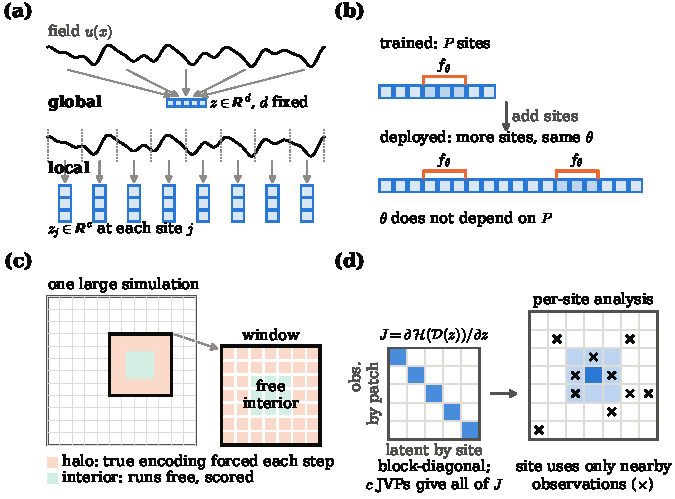
\includegraphics{figures/fig01_concept.pdf}
\caption{The idea in four panels. (a) A global latent compresses the
whole field into one vector of fixed dimension $d$; a local latent field
assigns $c$ channels to the site of each patch. (b) Because every
operator is shared across sites and reads a bounded neighbourhood, the
trained parameters $\theta$ do not depend on the number of sites, and the
model is deployed on a larger domain by adding sites. (c) Training on
windows of one large simulation: at every step of a training rollout the
halo of the window is overwritten by the true encoding, the interior
runs free, and only the interior is scored, so the loss is exactly that
of a limited-area model (Proposition~\ref{prop:halo}). (d) With a
per-patch decoder, the Jacobian of the observations with respect to the
latent is block-diagonal, so it is obtained from $c$ forward-mode
derivatives at any domain size and each site can be analysed from nearby
observations alone (Part~II).}
\label{fig:concept}
\end{figure*}

\para{Contributions.}
\begin{itemize}
\item \emph{A local latent field for extensive chaos}
  (Sec.~\ref{sec:method}): weight-shared encoder, decoder and propagator
  of finite reach, exactly translation-equivariant, with a parameter
  count independent of the domain size: about $135{,}000$ parameters describe
  the local law once, and the same parameters run domains of any size.
\item \emph{Zero-shot transfer validated by Lyapunov spectra}
  (Sec.~\ref{sec:results1d}). Trained at $L=100$, a 1D KS model reproduces
  the true $\DKY$ to within $0.2$--$1.2\%$ from $L=50$ to $L=400$, three
  training seeds agree to within $1.2\%$, and the whole positive part of
  its Lyapunov spectrum collapses onto the truth's.
\item \emph{The training distribution decides transfer}
  (Sec.~\ref{sec:results2d}). Trained on a small periodic box, the same
  architecture misses $\DKY$ by $15$--$38\%$ on larger domains in three of
  four cases in two 2D systems, and adding non-local inputs makes this
  worse. Trained on
  windows of one large domain, with the window's boundary driven by the
  simulation, the final models are within $0.6$--$2\%$ of the truth in 2D
  KS and $1$--$9\%$ in Kolmogorov flow at the two stronger drags, and
  within the truth's own uncertainty in their scaling with domain size;
  the weakest drag is harder. The window training is a learned
  limited-area model, and we prove it trains that problem exactly.
\item \emph{What fails, and why} (Sec.~\ref{sec:failure}): softmax
  attention, short rollouts and squared-error damping, with a lemma that
  connects the last to an underestimate of $\DKY$, and a model-selection
  rule that uses no ground truth.
\item \emph{Exactly local latent data assimilation}
  (Sec.~\ref{sec:da_results}). With a per-patch decoder the latent
  observation Jacobian is block-diagonal and is obtained from as many
  forward passes as there are channels, at any domain size, so a per-site
  ensemble filter in latent space is exact. Running it on four copies of the
  patch lattice shifted by half a patch and blending them removes the error
  tied to the lattice and lowers the analysis error by about $30\%$ without
  retraining; the gain comes from the offsets, not from the extra members.
  With one model trained only on noisy fields, and one setting, the analysis
  error is $0.30$--$0.33$ on every domain from $44^2$ to $440^2$, against $0.82$ for
  interpolating the observations, while an unlocalized filter fails once
  the attractor has more unstable directions than the ensemble has members.
\item \emph{Learned versus physics-based filters} (Sec.~\ref{sec:da_model_error}).
  Against a physics-based ensemble filter whose model is wrong, given
  online parameter estimation and bias correction, the latent filter loses
  when the model error is small or correctable and wins when it is large or
  structural. The outcome is predicted by one number, the part of the
  physical model's one-cycle forecast error that bias correction cannot
  remove: the crossover is near a sixth of the observation error.
\end{itemize}

What is not new should be said as clearly. Localized reduced models of KS
were built from wavelets a quarter century ago \citep{wittenberg2001},
learned models of KS have reproduced Lyapunov spectra at a single size
\citep{pathak2017,vlachas2020,ozalpmagri2025}, and convolutional
surrogates have been run on larger domains than they were trained on
\citep{barsinai2019,kochkov2021}. Section~\ref{sec:background} places our
results among these. The contrast with minimal flow units, which are
non-extensive by construction and where a global latent vector works
well \citep{constanteamores2025}, is the one-sentence summary of when a
field-valued latent is needed.

The paper has two parts. Part~I (Secs.~\ref{sec:method}--\ref{sec:results2d}
and \ref{sec:failure}) concerns the dynamics: the model and its
properties, the systems and the precision of their ground truth, transfer
in one and two dimensions, and the failure modes. Part~II
(Sec.~\ref{sec:da_results}) concerns data assimilation. Section~\ref{sec:discussion}
discusses what transfer requires and the limitations of this study.

%======================================================================
\section{Background and related work}
\label{sec:background}
%======================================================================

%----------------------------------------------------------------------
\subsection{Extensive chaos and its Lyapunov analysis}
\label{sec:bg_extensive}
%----------------------------------------------------------------------

A spatially extended system is extensively chaotic when the dimension of
its attractor grows in proportion to its volume. Ruelle conjectured that
the Lyapunov spectrum of turbulence has a large-volume limit, a density of
exponents per unit volume \citep{ruelle1982}; numerical studies of
coupled map lattices established such a limit for lattice maps
\citep{livi1986,isola1990}, and \citet{bunimovichsinai1988} proved
related results for weakly coupled maps. For the Kuramoto--Sivashinsky
equation extensivity of the Kaplan--Yorke dimension $\DKY$
\citep{kaplanyorke1979} was found by \citet{manneville1985}, and
\citet{edson2019} give $\DKY\approx0.226L-0.16$ for $L\gtrsim80$.
\citet{egolfgreenside1994} showed that extensivity holds in a
representative pattern-forming system but that the dimension density is
not set by the two-point correlation length, so the length that controls
it must be found by other means. Not every degree of freedom counted by
$\DKY$ is local: \citet{yang2009} separate a finite set of ``physical''
Lyapunov modes from the rest in KS, and \citet{takeuchi2009} show that
large chaotic systems can carry collective modes. Spectra are computed
with the method of \citet{benettin1980}.

Two results are especially close to our question. The first is that a
lattice spectrum computed on a small subsystem, suitably rescaled,
predicts the spectrum, $\DKY$ and entropy of the large system
\citep{carretero1999}. A trained local model is a learned lattice map, so
this is the dynamical-systems basis for expecting that a model trained
on a small domain can reproduce the dimension of a large one. The second
is that perturbations in spatiotemporal chaos spread at a finite speed,
measured by comoving (velocity-dependent) Lyapunov exponents
\citep{kaneko1986,deisslerkaneko1987}. We measure this speed for 1D KS
but find that it does not set the reach a model needs
(Sec.~\ref{sec:receptive}).

Two-dimensional flows add a complication. Without large-scale
dissipation the inverse energy cascade piles energy into the largest
scale the domain allows
\citep{kraichnan1967,smithyakhot1993,boffettaecke2012}, so statistics,
and the dimension, depend on the domain size. Linear drag arrests the
cascade, which is why we use Kolmogorov flow with drag
(Sec.~\ref{sec:kolmogorov}). The most closely related dimension study of
Kolmogorov flow, \citet{kolmogorovregimes2026}, computes $\DKY$ across
Reynolds numbers and forcing wavenumbers in a fixed box without drag.

%----------------------------------------------------------------------
\subsection{Learned surrogates of spatiotemporal chaos}
\label{sec:bg_surrogates}
%----------------------------------------------------------------------

\para{Global latent models.} The common design encodes the whole field
into one latent vector and learns its evolution, for example with
autoencoders and neural ordinary differential equations on an inertial
manifold \citep{linotgraham2020,linotgraham2022}, or with convolutional
autoencoders and echo state networks \citep{racca2023}. Such models are
tied to the size of the domain they were trained on.

\para{Lyapunov-level validation.} Learned models of KS have been shown to
reproduce its Lyapunov spectrum: a reservoir computer at $L=60$
\citep{pathak2017}, reservoir and recurrent networks
\citep{vlachas2020}, and latent models with their covariant Lyapunov
vectors \citep{ozalp2023,ozalpmagri2025}. Each validation is at the
single domain size the model was trained on.

\para{Local models of large domains.} Parallel reservoir computers
forecast KS on large domains by assigning one reservoir to each
subdomain \citep{pathak2018}. For the translation-invariant case the
reservoirs can share their weights, but a new set is trained for each
domain size and the Lyapunov exponents reported are those of the PDE,
not of the model. Patch-decomposed autoencoders with neural ODEs model
KS and Kolmogorov flow with low-dimensional latents per patch, coupled to
their neighbours \citep{constanteamores2024}; each domain size has its
own model, and validation uses short-time tracking and flow statistics.
In a minimal flow unit, which is non-extensive by construction, a single
global latent suffices \citep{constanteamores2025}; this contrast is the
reason a field-valued latent is needed for extensive chaos.

\para{Deployment on larger domains.} Convolutional models of PDEs are
translation-equivariant and can be run on domains larger than their
training domain. Learned discretizations trained on a small periodic
domain run on a ten times larger one \citep{barsinai2019}, learned
corrections to a coarse Navier--Stokes solver perform equally well on a
Kolmogorov domain twice as large \citep{kochkov2021}, learned coarse
simulators generalize qualitatively to larger KS domains
\citep{stachenfeld2022}, a pre-trained local neural operator is reused on
unseen geometries \citep{li2024lno}, and transformer operators with a
locality bias transfer to domains up to ten times larger per axis
\citep{devilleroche2026}. These studies validate by short-time error or
by statistics, not by the dimension of the attractor; the last one uses
non-chaotic benchmarks. Training fully convolutional networks on image
crops and applying them to whole images \citep{long2015} is the
computer-vision form of the same idea; generalization to finer
resolution, a different question, does not follow from it
\citep{sakarvadia2026}. Local neural-field latents have been reported to
fail on KS, with the decoder as the bottleneck \citep{aroma2024}.

\para{Limited-area models.} Our window training is a learned
limited-area model: the interior evolves freely while the boundary zone
is overwritten by the parent solution, a zero-width version of the
relaxation zone of \citet{davies1976}, with the known risks of
lateral-boundary errors \citep{warner1997}. Graph-based neural weather
models have been built for limited areas with boundary forcing
\citep{oskarsson2023}.

\para{Rollout training.} Training on multi-step rollouts stabilizes
learned solvers \citep{brandstetter2022,lippe2023}, but squared-error
rollouts blur the forecast toward the conditional mean
\citep{lam2023graphcast,bonavita2024}, and training objectives that match
invariant measures or dynamical invariants have been proposed to counter
it \citep{jiang2023,schiff2024,platt2023}. Training with input noise is
equivalent to a Jacobian penalty \citep{bishop1995}. Section~\ref{sec:objective}
connects both effects to an underestimate of $\DKY$.

%----------------------------------------------------------------------
\subsection{Latent and localized ensemble data assimilation}
\label{sec:bg_da}
%----------------------------------------------------------------------

Ensemble Kalman filters
\citep{burgers1998,houtekamermitchell1998,whitakerhamill2002} estimate
forecast covariances from a small ensemble, and localization makes them
work when the ensemble is much smaller than the state: by tapering the
covariance \citep{houtekamermitchell2001,gaspari1999}, by analysing each
grid point from nearby observations
\citep{ott2004,hunt2007}, or by correcting sampling error without a
distance \citep{anderson2012}. The two common localizations are related
but not equivalent \citep{sakovbertino2011,greybush2011}. The case for
localization rests on local low dimensionality \citep{patil2001}: the
forecast errors within a region span few directions. Without
localization, a filter needs at least as many members as there are
unstable and neutral directions
\citep{trevisan2004,gurumoorthy2017,bocquetcarrassi2017}; for a
deterministic filter on Lorenz-96 the minimum is $N_+ + 1$, with $N_+$ the
number of positive exponents \citep{takeda2026}. Particle flow filters
offer a nonlinear alternative \citep{huvanleeuwen2021}.

Filters in learned latent spaces have been built with global latents and
no localization
\citep{peyron2021,chen2023roadenkf,pasmans2025,tong2026laeenkf}. The
reduced-order autodifferentiable ensemble Kalman filter of
\citet{chen2023roadenkf}, which includes KS among its tests, explicitly
does not pursue covariance localization, and the latent autoencoder
filter of \citet{tong2026laeenkf} lists it as future work. Learned
corrections to ensemble filters can outperform a tuned local ensemble
transform Kalman filter (LETKF) on KS \citep{bach2025}, and latent
score-based filters note that a generic encoding destroys the local
structure that LETKF-type methods exploit \citep{si2025latentensf}. That observation is the starting point of
Part~II: a latent built to be local keeps that structure, exactly.

%----------------------------------------------------------------------
\subsection{What is and is not new here}
\label{sec:bg_novelty}
%----------------------------------------------------------------------

That KS admits localized reduced models is not new:
\citet{wittenberg1999} showed with wavelets that its dynamics are
localized in both space and scale, and \citet{wittenberg2001} built
localized low-dimensional models from short periodized subsystems,
arguing that they are minimal models for arbitrarily large domains. That
learned models can reproduce Lyapunov spectra, that local models can be
run on larger domains, and that localization makes ensemble filters work
with small ensembles are each established. Table~\ref{tab:prior_work}
summarizes the closest work. What we add is the combination: a learned,
weight-shared local latent field whose zero-shot extensions are checked
against the true Lyapunov spectra at several domain sizes in three
systems; a training procedure on windows of one simulation, with a proof
that it trains the limited-area problem exactly; and a latent observation
operator that is exactly local, so that a localized ensemble filter in
latent space is exact and keeps working at any domain size.

\begin{table*}[htbp]
\caption{Closest prior work. ``Local'': weight-shared operators of finite
reach; ``other sizes'': one trained model evaluated on domains of another
size; ``Lyapunov'': the model's own Lyapunov spectrum or $\DKY$ compared
with the truth; ``windows'': trained on windows of a larger domain with
boundary forcing; ``local DA'': localized ensemble data assimilation in a
learned latent space. $\circ$: partly (see text).}
\label{tab:prior_work}
\widetabular{lcccccc}{
work & learned & local & other sizes & Lyapunov & windows & local DA \\
\hline
\citet{carretero1999} & --- & \checkmark & \checkmark & \checkmark & --- & --- \\
\citet{wittenberg2001} & --- & \checkmark & $\circ$ & --- & $\circ$ & --- \\
\citet{pathak2017,vlachas2020} & \checkmark & --- & --- & \checkmark & --- & --- \\
\citet{ozalpmagri2025} & \checkmark & --- & --- & \checkmark & --- & --- \\
\citet{pathak2018} & \checkmark & $\circ$ & --- & --- & $\circ$ & --- \\
\citet{constanteamores2024} & \checkmark & $\circ$ & --- & --- & --- & --- \\
\citet{barsinai2019,kochkov2021} & \checkmark & \checkmark & \checkmark & --- & --- & --- \\
\citet{devilleroche2026} & \checkmark & \checkmark & \checkmark & --- & --- & --- \\
\citet{oskarsson2023} & \checkmark & $\circ$ & --- & --- & \checkmark & --- \\
\citet{chen2023roadenkf,tong2026laeenkf} & \checkmark & --- & --- & --- & --- & --- \\
This work & \checkmark & \checkmark & \checkmark & \checkmark & \checkmark & \checkmark \\}
\end{table*}

%======================================================================
\section{Method}
\label{sec:method}
%======================================================================

This section defines the model, states the structural properties that
make domain transfer and localized data assimilation possible, and fixes
the training and evaluation protocols used for every result in
Secs.~\ref{sec:results1d}--\ref{sec:failure}. Proofs of the
propositions are in Appendix~\ref{app:proofs}; numerical settings for
each system are in Appendix~\ref{app:architecture}.

%----------------------------------------------------------------------
\subsection{Setting and notation}
\label{sec:notation}
%----------------------------------------------------------------------

We consider a dissipative PDE $\partial_t u = N(u)$ for a scalar field
$u(\bm{x},t)$ on a periodic domain $\Omega$, either an interval of length
$L$ or a rectangle $L_x\times L_y$. The field is sampled on a uniform grid
of spacing $\Delta x$ and observed at snapshot interval $\Delta t$, giving
a discrete-time state $u_n = u(\cdot, n\Delta t)$. All fields are
standardized with a single mean and standard deviation computed on the
training data.

The domain is tiled by non-overlapping square \emph{patches} of
$p$ grid points per side, so that each patch has physical size
$h = p\,\Delta x$. The patch centres form a periodic \emph{site lattice}
$\Lat$ with $P = |\Lat|$ sites ($P = L/h$ in one dimension,
$P = (L_x/h)(L_y/h)$ in two). We write $\dist(j,k)$ for the periodic
(toroidal) distance between sites in units of the site spacing, and
$\Shift_s$ for the shift of a lattice field by $s\in\Z^{\dim}$ sites. A
shift of the physical field by $s$ whole patches is written
$\Tr_{s} u(\bm{x}) = u(\bm{x} - s h)$.

Two quantities set the scale of everything that follows. The first is
the number of active degrees of freedom, measured by the Kaplan--Yorke
dimension
\begin{equation}
  \DKY = k + \frac{\sum_{i=1}^{k}\lambda_i}{|\lambda_{k+1}|},
  \qquad
  k = \max\Big\{\, j : \textstyle\sum_{i=1}^{j}\lambda_i \ge 0 \Big\},
  \label{eq:dky}
\end{equation}
where $\lambda_1\ge\lambda_2\ge\cdots$ are the Lyapunov exponents
\citep{kaplanyorke1979}. The second is how $\DKY$ grows with domain
size. In \emph{extensive} chaos it grows in proportion to the volume,
\begin{equation}
  \DKY(\Omega) = \rho\,|\Omega| + o(|\Omega|),
  \label{eq:extensive}
\end{equation}
with a density $\rho$ that does not depend on $|\Omega|$
\citep{ruelle1982,manneville1985,egolfgreenside1994}. For the 1D
Kuramoto--Sivashinsky (KS) equation, $\rho\approx0.22$ per unit length
\citep{edson2019}. Equation~\eqref{eq:extensive} is the property a
surrogate must reproduce to be usable on domains larger than the one it
was trained on, and the property a fixed-size latent vector cannot
represent: its dimension is fixed at training time.

%----------------------------------------------------------------------
\subsection{Local latent fields}
\label{sec:local_field}
%----------------------------------------------------------------------

The latent state is a field on the site lattice,
\begin{equation}
  z = (z_j)_{j\in\Lat}, \qquad z_j \in \R^{c},
  \qquad \dlat = cP,
  \label{eq:latent_field}
\end{equation}
with $c$ channels per site. It is never flattened into an unstructured
vector except to call a library routine, and the flattening is always
site-major so that site identity is recoverable. The model has three
parts, each built only from operators that are applied identically at
every site and read a bounded neighbourhood.

\para{Encoder.}
The encoder $\E$ first maps each patch to a hidden vector by a strided
convolution whose kernel equals the patch (an exact, non-overlapping
patch embedding), then applies $n_e$ circular convolutions of radius
$r_e$ on the site lattice with GELU activations, and finally a
$1\times1$ convolution to $c-1$ channels. Channel $0$ is not learned: it
is the patch average of $u$,
\begin{equation}
  z_{j,0} = \frac{1}{|\text{patch } j|}\sum_{\bm{x}\in\text{patch } j} u(\bm{x}),
  \label{eq:anchor}
\end{equation}
which fixes one coordinate of the representation to a physical quantity
with the same meaning at every domain size. The output projection has
no bias: a per-channel offset shifts every site of the latent field by
the same constant, which the decoder can absorb and none of the training
losses constrains, so it drifts during training.

\para{Decoder.}
The decoder $\Dec$ mirrors the encoder: a $1\times1$ convolution from
$c$ channels to a hidden width, $n_d$ circular convolutions of radius
$r_d$, and a transposed convolution with kernel and stride equal to the
patch, which writes each site's hidden vector back onto its own patch.
The \emph{reach} of the encoder and decoder is $\Renc = r_e n_e$ and
$\Rdec = r_d n_d$ sites. When $\Renc=\Rdec=0$ the autoencoder is
\emph{per-patch}: site $j$'s latent is a function of patch $j$ alone,
and patch $j$ is reconstructed from $z_j$ alone. This is the canonical
autoencoder for the 2D systems (Sec.~\ref{sec:canonical_recipe}); the 1D
model uses $\Renc=\Rdec=6$ sites (Appendix~\ref{app:architecture}).

\para{Propagator.}
The latent dynamics are a residual map
\begin{equation}
  z^{n+1} = \Fp(z^{n}) = z^{n} + f_\theta(z^{n}),
  \label{eq:propagator}
\end{equation}
where $f_\theta$ (``local MLP'') embeds each site's $c$ channels to a
width $d_m$, applies $n_\ell$ blocks of the form
\begin{equation}
  \begin{aligned}
  a &\leftarrow a + \mathrm{Conv}_{w}\big(\mathrm{LN}(a)\big),\\
  a &\leftarrow a + \mathrm{MLP}\big(\mathrm{LN}(a)\big),
  \end{aligned}
  \label{eq:mixer_block}
\end{equation}
and projects back to $c$ channels per site. Here $\mathrm{Conv}_{w}$ is
a circular convolution of radius $w$ over the site lattice (kernel
$2w+1$ per axis), $\mathrm{LN}$ is layer normalization over channels at
each site, and $\mathrm{MLP}$ acts on each site independently. The token
mixer is an \emph{unconstrained linear} map of the neighbourhood: there
is no softmax normalization. Every self-attention propagator we tried
collapsed to a fixed point under free rollout (Sec.~\ref{sec:fail_attention});
replacing softmax attention by a linear mixer of the same radius removed
the collapse. The final projection is initialized to zero, so
$\Fp=\mathrm{id}$ at initialization and early rollouts are stationary
rather than divergent.

\para{Structural properties.}
All learned operators above are weight-shared and of finite radius on a
periodic lattice. Two consequences follow directly.

\begin{proposition}[Equivariance and size independence]
\label{prop:equivariance}
Let $\E$, $\Dec$ and $\Fp$ be built as above on a periodic lattice with at
least $2r+1$ sites along every axis on which a kernel of radius $r$ acts.
Then for every shift $s$ by a whole number of patches,
\begin{equation}
  \E\circ\Tr_{s} = \Shift_s\circ\E, \qquad
  \Dec\circ\Shift_s = \Tr_{s}\circ\Dec, \qquad
  \Fp\circ\Shift_s = \Shift_s\circ\Fp,
  \label{eq:equivariance}
\end{equation}
exactly, and the parameter vector $\theta$ of all three maps is the same
for every $P$.
\end{proposition}

\begin{corollary}[Transfer by adding sites]
\label{cor:transfer}
Hold $\Delta x$ and $p$ (hence $h$) fixed. Then a parameter vector
$\theta$ trained on any domain defines, without modification, a model on
every periodic domain whose side lengths are multiples of $h$, with
$P$ and $\dlat=cP$ growing in proportion to $|\Omega|$.
\end{corollary}

Corollary~\ref{cor:transfer} is the zero-shot transfer evaluated
throughout this paper: a checkpoint trained at one size is loaded at a
new $(N_x,P)$, with every weight copied unchanged. A global latent vector
admits no such map, because its bottleneck and propagator are tied to
one value of $\dlat$.

A local model is also extensive by construction, which explains both
what transfer can achieve and how it fails.

\begin{remark}[Local models are extensive]
\label{rem:extensive_model}
For translation-invariant lattice maps of finite range the Lyapunov
spectrum is expected, and found numerically, to have a thermodynamic
limit: the exponents, indexed per site, converge to a density as
$P\to\infty$
\citep{ruelle1982,livi1986,isola1990}; rigorous results exist for weakly
coupled maps \citep{bunimovichsinai1988}. For a local model this gives
$\DKY^{\text{model}}(\Omega) = \rho_\theta|\Omega| + o(|\Omega|)$ with a
density $\rho_\theta$ fixed by the trained weights, and the spectrum of a
small lattice already predicts that of a large one, as
\citet{carretero1999} showed for coupled map lattices. A local model can
therefore match the true density $\rho$. Its finite-size corrections,
however, are set by its own reach $\Rprop h$, not by the physics, so it
need not reproduce the true system's departures from
Eq.~\eqref{eq:extensive} on domains comparable to that reach. We use this
as an interpretive principle rather than a theorem about our networks: in
the results below the model's density is nearly constant across sizes,
and its largest errors occur where the domain is only a few reaches
wide.
\end{remark}

%----------------------------------------------------------------------
\subsection{Receptive fields and locality}
\label{sec:receptive}
%----------------------------------------------------------------------

The output of the encoder at site $j$ depends on patches within
$\Renc$ sites of $j$; one propagator step at site $j$ depends on latent
sites within $\Rprop = w\,n_\ell$ sites; the decoder output on patch $j$
depends on latent sites within $\Rdec$. After $k$ propagator steps,
the decoded field on patch $j$ depends on the initial field within
\begin{equation}
  R_k = \Renc + k\,\Rprop + \Rdec
  \label{eq:light_cone}
\end{equation}
sites. Unit tests confirm each reach on the implemented maps by masking
their Jacobians.

How large must $\Rprop$ be? For a dissipative PDE such as KS the exact
one-step map has an unbounded domain of dependence, but its influence
decays rapidly with distance, so the relevant quantity is an
\emph{interaction range}: the distance beyond which neighbouring values
no longer improve a one-step prediction. We measure it directly on the
1D latent. A single quadratic stencil, shared by all sites, that predicts
each site's one-step increment from the sites within a half-width $w$
explains $58\%$ of the variance at $w=1$, $82\%$ at $w=2$, $88\%$ at
$w=3$ and saturates at $90\%$ from $w=4$ on, the value it also reaches
with access to the whole ring (a linear stencil explains at most
$2.5\%$ at any width; Fig.~\ref{fig:appendix_panels}(c)). The interaction range of the 1D dynamics at
$\Delta t=1$ is therefore three to four sites, $19$--$25$ length units, or
two to three pattern wavelengths. The trained propagator's reach of six
sites ($37.5$ units) covers it with a margin; the 2D models' six-site
reach spans about four pattern wavelengths in 2D KS ($33$ units) and
three forcing wavelengths in Kolmogorov flow ($4.7$ units).

A second, more familiar length is set by the speed at which
perturbations spread. In spatiotemporal chaos this speed is finite and
is characterized by the largest velocity $v_*$ with a positive comoving
(velocity-dependent) Lyapunov exponent
\citep{kaneko1986,deisslerkaneko1987}. For 1D KS we measure
$v_*=1.26\pm0.04$ length units per time unit (150 trajectories), so a
perturbation spreads $v_*\Delta t\approx1.3$ units, a fifth of a site,
during one snapshot interval. This is a lower bound on the reach a
propagator needs, and it is far from binding here: the interaction range
is set by how far the one-step map couples values, not by how far
perturbations travel. The same distinction applies to localization in
data assimilation (Sec.~\ref{sec:da_method}): an analysis increment at
site $j$ must reach every site that the decoder or the forecast couples to
$j$. With a per-patch decoder the decoder contributes nothing, and the
light-cone term $v_*\Delta t_{\mathrm{win}}$ over an assimilation window
of five snapshots is about $6$ length units in 1D, far inside the
localization radii we use.

%----------------------------------------------------------------------
\subsection{Training on windows of a large domain}
\label{sec:crop_training}
%----------------------------------------------------------------------

A model trained on a small periodic box sees only that box's statistics,
and a propagator whose reach covers most of the box can exploit the
periodic wrap-around, a self-interaction that does not exist on a larger
domain. In our 2D experiments this happened: a propagator with
$\Rprop=6$ trained on an $8$-site periodic ring covers $75\%$ of it, and
such models fail to transfer (Sec.~\ref{sec:box_vs_window}). We instead
simulate one large periodic domain and train only on random rectangular
windows (\emph{crops}) of it. A crop has no boundary condition: its
edges are open, and the training losses are restricted to the sites a
light-cone argument certifies.

\para{Stage A: autoencoder.}
A crop of $W$ sites per cropped direction is encoded and decoded. Sites
within $\Renc+\Rdec$ of a crop edge are excluded from the
reconstruction loss, because padding at the edge reaches them. For a
per-patch autoencoder this margin is zero.

\para{Stage B: propagator with a forced halo.}
The trained encoder is frozen and applied to many crops of every training
trajectory at every time, giving a bank of latent crop trajectories.
The outer $\Renc$ sites per cropped side are dropped, since their
encoding saw padding. The remaining strip is split into a \emph{halo}
of $\eta$ sites per side and a \emph{free interior} $I$. A training
rollout starts from the true encoding, applies the propagator, and after
every step overwrites the halo with the true encoding at that time; only
the interior is scored. This is the construction of a limited-area
forecast model driven by lateral boundary data from a parent run.

\begin{proposition}[Forced-halo exactness]
\label{prop:halo}
Let $\eta\ge\Rprop$. Then for every rollout length $k$, the forced-halo
prediction on the free interior equals the prediction of the same
weights on any larger periodic domain containing the crop, in which every
site outside $I$ is set to its true value at every step. If
$\eta<\Rprop$, the equality fails in general.
\end{proposition}

Proposition~\ref{prop:halo} says the crop loss is the loss of a
well-defined object, the model restricted to $I$ with exact lateral
boundary data, and that no padding artifact enters the gradient. It is
checked numerically (agreement to $10^{-6}$ for strips cropped in one
direction and $10^{-5}$ for windows cropped in both, and companion tests
that halos of $\Rprop-1$ and $\Rprop-2$ break it). The one
mismatch between training and deployment is that interior sites adjacent
to the halo see true neighbours in training and predicted neighbours on
the periodic deployment domain; it is confined to a strip of width
$\Rprop$.

For 2D Kuramoto--Sivashinsky, which is isotropic, crops are cut in both
directions, so no training sample contains a whole periodic direction.
For Kolmogorov flow, whose forcing depends on $y$, crops are strips in
$x$ that keep the full periodic height, and transfer grows the domain in
$x$ only.

%----------------------------------------------------------------------
\subsection{Training objective}
\label{sec:objective}
%----------------------------------------------------------------------

\para{Stage A.}
For a batch of crops with interior latents $\{z_j\}$ pooled over sites
and batch members, let $C = \Cov(z)\in\R^{c\times c}$ be their channel
covariance. The loss is
\begin{equation}
\begin{split}
  \mathcal{L}_A ={}&
  \big\|\,\Dec(\E(u)) - u\,\big\|^2_{I}
  + \wvar\,\frac1c\sum_{k=1}^{c}\big(C_{kk}-1\big)^2\\
  &- \wld\,\frac1c\log\det\!\big(C + \epsilon I_c\big),
\end{split}
  \label{eq:stageA}
\end{equation}
where $\|\cdot\|_I$ is the mean squared error over the unmasked interior.
The two regularizers do different jobs. The log-determinant barrier
penalizes any small eigenvalue of $C$, whether it comes from a channel
with small variance or from a channel that is nearly a linear combination
of others, so it prevents correlated (rank) collapse that a per-channel
penalty cannot see. It does not, however, constrain the overall scale:
it decreases when all eigenvalues grow together, and the encoder and
decoder can rescale against each other with no change in reconstruction.
The variance term anchors that scale. With $\wvar=0$ we observed the
variance diagnostic grow from $8\times10^{2}$ to $2.5\times10^{8}$ over
training while the reconstruction error stayed flat.

\begin{remark}[The barrier offset $\epsilon$ is not a numerical detail]
\label{rem:epsilon}
The barrier's force on an eigenvalue $\mu$ of $C$ is
$-\partial_\mu\log(\mu+\epsilon) = -1/(\mu+\epsilon)$. At initialization
the smallest eigenvalue of $C$ for our architecture is
$0.8$--$4.4\times10^{-3}$ (ten random seeds), so changing $\epsilon$
from $10^{-3}$ to $0$ changes the force on the weakest directions by a
factor of order one. Section~\ref{sec:fail_mse} shows that this choice
changes the trained model's dimension at large domain sizes as much as
the rollout length does.
\end{remark}

\para{Stage B.}
The propagator is trained on forced-halo rollouts of length $k$,
\begin{equation}
  \mathcal{L}_B = \frac1k\sum_{m=1}^{k}
  \big\|\hat z^{m} - z^{m}\big\|_{I}^{2},
  \quad \hat z^{0} = z^{0} + \xi,\ \xi\sim\mathcal N(0,\sigma^2 I),
  \label{eq:stageB}
\end{equation}
where $\hat z^{m}$ is the forced-halo prediction. The rollout length $k$
is ramped from $2$ to an intermediate value $\kmid$ over the first $58\%$
of training, then to its final value $\kmax$, and held there for the last
$30\%$; the input noise $\sigma$ is
annealed linearly from $0.10$ to $0.02$. Long free rollouts are needed:
short ones leave the free-running model under-constrained and produce
spurious, initial-condition-dependent regimes (Sec.~\ref{sec:fail_regimes}).
But long rollouts scored by mean squared error carry a known bias.

\begin{lemma}[Squared-error rollouts favour contraction]
\label{lem:mse}
Let $(z^0, z^k)$ be jointly distributed with finite second moments, and
let $\tilde z^0$ be the (possibly noisy) model input. Among all
measurable maps $\Phi$, the expected loss
$\Exp\|\Phi(\tilde z^0)-z^k\|^2$ is minimized by
$\Phi^\star(\tilde z^0)=\Exp[z^k\mid\tilde z^0]$, and
\begin{equation}
  \tr\Cov\big(\Phi^\star(\tilde z^0)\big)
  = \tr\Cov(z^k) - \Exp\,\tr\Cov\big(z^k\mid\tilde z^0\big).
  \label{eq:total_variance}
\end{equation}
\end{lemma}

The second term in Eq.~\eqref{eq:total_variance} is the forecast
uncertainty at lead $k$. In a chaotic system it is non-zero at every
$k>0$: input noise of variance $\sigma^2$ grows along the leading
direction as $\sigma^2 e^{2\lambda_1 k\Delta t}$ until it saturates at the
climatological variance. A propagator trained toward $\Phi^\star$ is
therefore rewarded for rollouts whose spread is smaller than that of
real trajectories, that is, for contracting along the most unstable
directions, and the reward grows with $k$. Our training horizons are
short in Lyapunov units: $\kmax\Delta t\,\lambda_1\approx1.1$ for 1D KS,
$0.5$--$0.65$ for 2D KS, and $0.2$--$1.0$ for Kolmogorov flow across the
three drags. The effect is therefore a bias that grows with $\kmax$,
not the collapse to the climatological mean that a horizon of many
Lyapunov times would produce. It is the mechanism behind the
``blurring'' of machine-learned weather models
\citep{lam2023graphcast,bonavita2024}, and for a learned surrogate it
predicts an underestimate of $\DKY$ that grows with $\kmax$, which is
what we observe (Sec.~\ref{sec:fail_mse}).

\begin{remark}[Input noise penalizes growth directly]
\label{rem:noise_penalty}
Training with input noise is, to leading order, a penalty on the
Jacobian of the trained map \citep{bishop1995}. Expanding
$\Phi(z+\xi)$ for small $\xi\sim\mathcal N(0,\sigma^2 I)$,
\begin{equation}
\begin{split}
  \Exp_\xi\big\|\Phi(z+\xi)-y\big\|^2
  ={}& \big\|\Phi(z)-y\big\|^2 + \sigma^2\big\|\partial_z\Phi(z)\big\|_F^2\\
  &+ \sigma^2\,\big(\Phi(z)-y\big)^{\!\top}\Delta_z\Phi(z) + O(\sigma^4),
\end{split}
  \label{eq:noise_penalty}
\end{equation}
where $\Delta_z\Phi$ is the vector of Laplacians of the components of
$\Phi$; the last term averages to zero at the regression optimum. For the
$k$-step map the Frobenius norm is at least the largest finite-time
growth factor, $\|\partial_z\Phi\|_F^2\ge e^{2\lambda^{(k)}_1 k\Delta t}$, so
input noise penalizes exactly the expansion that produces positive
exponents, with a strength $\sigma^2$. Rollout length and input noise
are two handles on one bias. The one run that raised both (rollouts to
$\kmax=32$ with terminal noise $0.05$ instead of $0.02$,
Sec.~\ref{sec:fail_regimes}) underestimates $\DKY$ by $4\%$, $13\%$ and
$14\%$ at $1\times$, $2\times$ and $3\times$.
\end{remark}

Rollouts that are too short fail in the opposite way
(Sec.~\ref{sec:fail_regimes}). We treat $\kmax$ and the noise schedule as
a trade-off between these two failure modes, not as quantities to
maximize.

%----------------------------------------------------------------------
\subsection{The canonical recipe}
\label{sec:canonical_recipe}
%----------------------------------------------------------------------

All 2D results in the main text share one architecture and training
procedure: a per-patch autoencoder ($\Renc=\Rdec=0$) with $c=6$ channels
(five learned and the anchor) and hidden width $32$; a local-MLP
propagator with $n_\ell=2$ blocks of radius $w=3$ ($\Rprop=6$ sites),
token width $d_m=32$ and MLP ratio $4$; training on crops of one large
domain with a forced halo $\eta=6$; and Stage~A for $8000$ steps and
Stage~B for $6000$--$9000$ steps with AdamW, linear warm-up and cosine
decay. The models differ in the rollout length $\kmax$ and in the
regularizer weights. $\kmax=32$ (2D KS and Kolmogorov flow at
$\alpha=0.025$) is the long-rollout setting introduced to suppress
spurious free-running regimes (Sec.~\ref{sec:fail_regimes}); the
$\alpha=0.05$ model is the earlier, independently verified $\kmax=12$
model, which a $\kmax=32$ retraining does not improve
(Sec.~\ref{sec:canonical_results}); and at $\alpha=0.1$, where $\kmax$ and
the barrier offset $\epsilon$ interact (Sec.~\ref{sec:fail_mse}), the
model ($\kmax=16$) was chosen among six variants by a rule that uses no
ground truth (Sec.~\ref{sec:canonical_results}).

The 1D model predates this recipe. It was trained on whole periodic
domains of $16$ sites with a full-reach encoder and decoder
($\Renc=\Rdec=6$, $c=3$), jointly with a short-horizon auxiliary
propagator, and with an additional penalty that favours spatial
coherence of the latent across neighbouring sites; the propagator was
then refined with rollouts up to $\kmax=12$. It transfers without crop
training (Sec.~\ref{sec:results1d}), so we did not retrain it with the 2D
recipe. Every setting of every model is listed in
Appendix~\ref{app:architecture}.

%----------------------------------------------------------------------
\subsection{Evaluation}
\label{sec:evaluation}
%----------------------------------------------------------------------

\para{Lyapunov spectra.}
We compute Lyapunov spectra by the Benettin algorithm with QR
reorthonormalization \citep{benettin1980}. For the true PDE, tangent
vectors are propagated with the exact Fr\'echet derivative of the
time-stepper in double precision. For a model, tangent vectors are
propagated through $\Fp$ by forward-mode automatic differentiation in
single precision and re-orthonormalized every 10 steps by a
double-precision QR on the CPU. The exponents are reported per unit
physical time, $\lambda_i = (n\Delta t)^{-1}\sum_{q}\log|R^{(q)}_{ii}|$,
where $R^{(q)}$ is the triangular factor of the $q$-th reorthonormalization
and $n$ the number of model steps. From each spectrum we report
$\lambda_1$, the number of positive exponents $n_+$, and $\DKY$. Each
model spectrum uses all $\dlat$
tangent directions, a warm-up of 200 steps and $n=2000$ steps (2000 time
units in 1D, 200 in 2D KS, 400 in Kolmogorov flow); the computation
raises an error if the cumulative sum in Eq.~\eqref{eq:dky} never turns
negative, so $\DKY$ is always bracketed rather than extrapolated. The
spectrum is that of the latent map; comparing it with the PDE's assumes
that the decoder is a smooth, injective map of the attractor, which the
agreement of the spectra themselves supports (Sec.~\ref{sec:results1d}).

A model trajectory starts from the encoding of a true on-attractor
state, standardized with the training statistics, and each model is
evaluated from three independent initial conditions per domain size
unless stated otherwise. A finite-time estimate from one initial
condition is a random quantity, for the model as for the truth: two runs
that differ only at round-off level (single versus double precision)
follow different chaotic trajectories. Averaged over three initial
conditions, double-precision propagation changes $\DKY$ by at most
$0.3\%$ in 1D and 2D KS and by $2.2\%$ in Kolmogorov flow at the native
size, where single runs scatter by $25\%$ across initial conditions; we
therefore report means over initial conditions and treat single-run
differences below that scatter as noise.

\para{Ground truth and its uncertainty.}
True spectra are computed after a spin-up of $100$--$200$ time units and
a warm-up of the tangent basis. For Kolmogorov flow we average over $120$
time units and record the running estimate of $\DKY$ at intermediate
times to check convergence; the window used for every truth value is
listed in Appendix~\ref{app:groundtruth}. The truth's finite-time $\DKY$ is
random in the same way as the model's. In Kolmogorov flow its
seed-to-seed spread is $4$--$13\%$ at the sizes we use
(Sec.~\ref{sec:truth_uncertainty}), comparable to many model errors, so we
report 2D results as scaling with domain size, with truth error bars,
rather than as single-point matches.

\para{Free-rollout statistics.}
Before any Lyapunov computation, each model is run freely for several
hundred time units and its field variance and energy spectrum, split
into large-scale and forcing-scale bands, are compared with the training
data or with the truth.
This check is cheap and detects drifting or multistable models that a
short teacher-forced validation loss does not (Sec.~\ref{sec:fail_regimes}).

%----------------------------------------------------------------------
\subsection{Latent ensemble data assimilation}
\label{sec:da_method}
%----------------------------------------------------------------------

Observations are taken of the physical field,
$y_n = \Hobs(u_n) + \nu_n$, $\nu_n\sim\mathcal{N}(0,R)$, where $\Hobs$
selects grid points on a regular sparse network. The filter state is
an ensemble $\{z^{(e)}\}_{e=1}^{\Nens}$ of latent fields, forecast with
$\Fp$ plus additive model noise, and the observation operator in latent
space is $h = \Hobs\circ\Dec$. We use three analysis schemes:
\begin{itemize}
\item a particle flow filter (the Gauss--Newton ``NAT'' variant of
  \citet{huvanleeuwen2021}), used in 1D;
\item a stochastic ensemble Kalman filter with perturbed observations
  \citep{burgers1998,houtekamermitchell1998} and Schur-product
  covariance localization \citep{houtekamermitchell2001}, with gain
  $K = (\rho\circ B)J^{\top}\big(J(\rho\circ B)J^{\top}+R\big)^{-1}$,
  where $B$ is the ensemble covariance, $\rho$ the taper, and $J$ the
  Jacobian of $h$ at the ensemble mean; used in 1D and 2D;
\item a per-site local ensemble Kalman filter in the local-analysis
  form of \citet{hunt2007}, with observation-space (R-)localization and
  the same perturbed-observation update: each site is updated from the
  observations within the taper's support, with each observation's error
  variance divided by its taper value; used in 2D.
\end{itemize}
The taper is the Gaspari--Cohn function \citep{gaspari1999} of the site
distance $\dist(j,k)$, with toroidal distance in 2D. As a distance-free
baseline we use sampling error correction (SEC), which replaces the
taper by a correction factor fitted offline from the sample correlation
\citep{anderson2012}.

The per-patch decoder makes the observation operator exactly local in
latent space.

\begin{proposition}[Block-diagonal observation Jacobian]
\label{prop:blockdiag}
Let $\Rdec=0$ and let $\Hobs$ select grid points. Then
$\partial h_i/\partial z_{j,k} = 0$ for every channel $k$ unless
observation $i$ lies in patch $j$. Consequently:
\begin{enumerate}
\item[(a)] the full Jacobian $J\in\R^{m\times\dlat}$ is recovered exactly
  from $c$ forward-mode Jacobian--vector products with the tangents
  $v^{(k)} = \sum_{j\in\Lat} e_{j,k}$, $k=1,\dots,c$, for any $P$ and any
  number of observations $m$;
\item[(b)] in the per-site filter with R-localization, with either the
  perturbed-observation or the ensemble-transform update, the analysis at
  site $s$ depends only on the ensemble at the sites that own an
  observation within the taper support of $s$, and no row of $J$ is
  truncated in computing it.
\end{enumerate}
\end{proposition}

Part (a) is a column colouring of $J$ in the sense of
\citet{curtis1974}: all columns belonging to the same channel can share
one colour, because no row has two non-zeros in such a group. With
$\Rdec>0$, row $i$ would have non-zeros at every site within $\Rdec$ of
its patch, the colouring would need $c(2\Rdec+1)^{\dim}$ colours, and the
per-site analysis in (b) would have to include those sites as well or
truncate $h$. Neither the cost of the colouring nor the memory of the
per-site filter depends on the domain size; the dense covariance-localized
filter, which forms $\dlat\times\dlat$ matrices, scales as $P^2$ in memory.

\para{How large an ensemble is needed.}
An ensemble filter needs enough members to span the directions along
which forecast errors grow. Without localization these are the unstable
directions of the whole attractor, so $\Nens$ must grow with $\DKY$ and
therefore with $|\Omega|$. With localization, each local analysis only
needs to span the unstable directions active inside the taper support
$A_{\mathrm{loc}}$ \citep{patil2001,ott2004}, which suggests
\begin{equation}
  \Nens \gtrsim \rho\,|A_{\mathrm{loc}}|,
  \label{eq:nens_local}
\end{equation}
independent of the total domain size. For 1D KS with the taper used in
Sec.~\ref{sec:da_results} (support radius $6$ sites of length $6.25$),
Eq.~\eqref{eq:nens_local} gives $\Nens\gtrsim 0.22\times75\approx17$.
Combined with Corollary~\ref{cor:transfer}, this is the reason to expect a
transferred local model to keep a fixed-size filter useful as the domain
grows, while an unlocalized filter of the same size degrades.

%======================================================================
\section{Systems, data and ground truth}
\label{sec:systems}
%======================================================================

We use three periodic, scalar, spatiotemporally chaotic systems of
increasing difficulty: the one-dimensional Kuramoto--Sivashinsky (KS)
equation, its two-dimensional isotropic generalization, and
two-dimensional Kolmogorov flow with linear drag. All three are
integrated in Fourier space with a fourth-order exponential time-differencing
Runge--Kutta scheme (ETDRK4), with the coefficients evaluated by the
contour-integral method of \citet{kassam2005} (32 points), in double
precision on the CPU. Table~\ref{tab:systems} collects the parameters,
Table~\ref{tab:truth} the ground-truth Kaplan--Yorke dimensions, and
Appendix~\ref{app:groundtruth} the full protocol and the solver
validation. Figure~\ref{fig:systems} shows each system on the domain its
models are trained on.

\begin{figure*}[htbp]
\centering
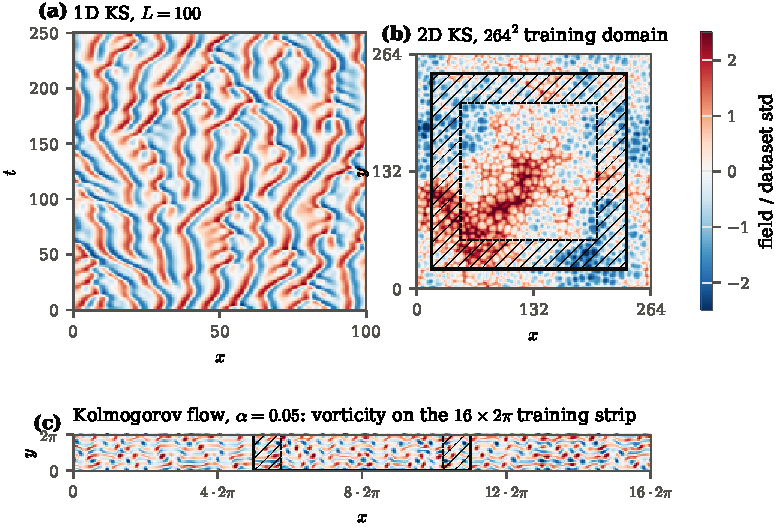
\includegraphics{figures/fig02_systems.pdf}
\caption{The three systems on their training domains, standardized by
the training standard deviation. (a) 1D KS at $L=100$: 250 time units
of one training trajectory. (b) 2D KS: one snapshot on the $264^2$
periodic domain whose windows train the 2D KS model; the outlined square
is one $40\times40$-site training window, its forced halo (six sites)
hatched and its free interior inside the dashed line. (c) Kolmogorov flow
at $\alpha=0.05$: vorticity on the $16\times2\pi$ by $2\pi$ training strip,
with one 48-site window spanning the full height and its six-site halo in
$x$. Cells of a fixed size fill the 1D and 2D KS domains, and the
Kolmogorov vortices are organized by the forcing at wavenumber 4 in
$y$; in each case the domain holds many independent copies of the local
dynamics, which is what window training samples.}
\label{fig:systems}
\end{figure*}

%----------------------------------------------------------------------
\subsection{One-dimensional Kuramoto--Sivashinsky}
\label{sec:ks1d}
%----------------------------------------------------------------------

The KS equation \citep{kuramoto1976,sivashinsky1977},
\begin{equation}
  u_t + u u_x + u_{xx} + u_{xxxx} = 0, \qquad x\in[0,L),
  \label{eq:ks1d}
\end{equation}
has a linear growth rate $k^2-k^4$ that is positive for $|k|<1$ and
largest at $k=1/\sqrt2$, which sets a pattern wavelength of
$2\sqrt2\,\pi\approx8.9$. For $L$ large compared with this length the
dynamics are extensively chaotic, with $\DKY\approx0.226L$ minus a
small offset \citep{manneville1985,edson2019}. We train at $L=100$ on a
grid of $256$ points ($\Delta x = 0.39$), with solver step $0.05$ and
snapshot interval $\Delta t=1.0$. The training set has 60 independent
trajectories (50 training, 10 validation) of 250 time units each, after
a spin-up of 500 time units.

Ground truth is computed at $\Delta x = 100/1024$, four times finer than
the training grid, to keep the solver error well below the model error,
with averaging windows of 1200--2000 time units (100 or more Lyapunov
times for $L\ge50$). At $L=100$ the reference value is $\DKY=22.5$,
inside the range $[21,24]$ reported in the literature, with
$\lambda_1=0.090$ and 12 positive exponents; \citet{edson2019} give
$\DKY\approx0.226L-0.16$ for $L\gtrsim80$, i.e.\ $22.4$. At $L=22$ our
solver gives $\DKY=5.26$ and $\lambda_1=0.049$, against $5.20$ and $0.043$
from \citet{edson2019} and a leading exponent of $0.048$ from
\citet{cvitanovic2010}. The transfer sizes $L=25,50,200,400$ give the
densities in Table~\ref{tab:truth}: $\DKY/L$ lies between $0.224$ and
$0.226$ for every $L\ge50$, while at $L=25$, close to the onset of
chaos, $\lambda_1\approx0.001$ and the density falls to about $0.07$.

%----------------------------------------------------------------------
\subsection{Two-dimensional Kuramoto--Sivashinsky}
\label{sec:ks2d}
%----------------------------------------------------------------------

The isotropic 2D generalization,
\begin{equation}
  u_t + \nabla^2 u + \nabla^4 u + \tfrac12|\nabla u|^2 = 0,
  \qquad (x,y)\in[0,L)^2,
  \label{eq:ks2d}
\end{equation}
has the same linear operator, now unstable on the ring $|\bm k|<1$
\citep{kalogirou2015}. Unlike the 1D equation, its nonlinearity is not a
total derivative and drives the spatial mean of $u$. The mean carries
no dynamical information (only gradients of $u$ enter the right-hand
side), so we project the $\bm k=0$ mode out after every step, in the
base trajectory and in every tangent vector. All runs use solver step
$0.02$, snapshot interval $\Delta t=0.1$ and grid spacing
$\Delta x = 0.344$ ($128$ points at $L=44$).

The training data are four trajectories (plus one for validation) of
25 time units on a single periodic domain of side $264=6\times44$
($768^2$ points), after a spin-up of 200 time units. Models are crop-trained
on this domain (Sec.~\ref{sec:crop_training}) and evaluated on square
periodic boxes of side $44$, $66$ and $88$. Ground truth exists at $44^2$
(three runs, $\DKY=80.7$--$83.6$, mean $82.0$, 42--44 positive exponents)
and $66^2$ (two runs, $185.6$ and $192.5$, mean $189.1$, 93--101 positive
exponents). The mean densities, $0.0424$ and $0.0434$ per unit area,
differ by $2.5\%$, inside the spread of the individual runs; we did not
compute a truth at $88^2$, where the expected dimension (about 330) would
need more than 500 tangent directions.

%----------------------------------------------------------------------
\subsection{Kolmogorov flow with linear drag}
\label{sec:kolmogorov}
%----------------------------------------------------------------------

Two-dimensional incompressible flow in vorticity form,
\begin{equation}
\begin{gathered}
  \omega_t + \bm u\cdot\nabla\omega = \nu\nabla^2\omega - \alpha\,\omega + f(y),\\
  \bm u = (\psi_y,-\psi_x),\qquad \nabla^2\psi=-\omega,
\end{gathered}
  \label{eq:kolmogorov}
\end{equation}
on $[0,L_x)\times[0,2\pi)$, with forcing
$f(y) = -(\nu n^2+\alpha)\,n\cos(ny)$. This forcing makes
$\bm u = (\sin ny, 0)$ an exact steady solution for every $\alpha$, which
gives an exact test of the solver (Appendix~\ref{app:groundtruth}).
We use $n=4$ and $\nu=0.01$, and three drag coefficients
$\alpha\in\{0.025,0.05,0.1\}$. We quote a Reynolds number
$Re=\sqrt{f_0}/\nu$ built from the velocity forcing amplitude
$f_0=\nu n^2+\alpha$ on a $2\pi$ box; this is the definition of
\citet{kolmogorovregimes2026} applied to our forcing, and coincides with
theirs for $\alpha=0$ (their flows have no drag). Our three drags give
$Re\approx43$, $46$ and $51$.

The drag is what makes the flow usable for domain transfer. Without it,
the two-dimensional inverse energy cascade accumulates energy at the
largest scale the box allows
\citep{kraichnan1967,smithyakhot1993,boffettaecke2012}, so the
statistics depend on the domain size and the dimension cannot be
extensive. With drag, the dimension per $2\pi\times2\pi$ box changes
by at most about $20\%$ between one and three boxes at every $\alpha$ we
use (Table~\ref{tab:truth}), comparable to the uncertainty of the
single-run truths (Sec.~\ref{sec:truth_uncertainty}); without drag the
flow condenses into a domain-scale mean state.

The forcing singles out $y$: the equation is translation-invariant in
$x$ and invariant in $y$ only under shifts by the forcing period $2\pi/n$.
We therefore keep the height fixed at $2\pi$ and grow the domain in $x$
only, to $2\times$ and $3\times$ the square box. Kolmogorov results are
statements about widening the channel, not about growing its area in
both directions; the 2D KS results are the isotropic test. All runs use
grid spacing $2\pi/128$, solver step $0.01$ and snapshot interval
$\Delta t=0.2$. Training data come from a domain of width $16\times2\pi$
($2048\times128$ points), four training and one validation trajectory of
40 time units per drag value, after a spin-up of 100 time units.

%----------------------------------------------------------------------
\subsection{How precise is the ground truth?}
\label{sec:truth_uncertainty}
%----------------------------------------------------------------------

Every comparison in this paper is between a model's $\DKY$ and a
finite-time estimate of the true $\DKY$ from one or a few initial
conditions. The precision of that estimate differs greatly between the
systems, and it limits what can be claimed.

\para{1D KS.} Windows of 1200--2000 time units span 100 or more
Lyapunov times for $L\ge50$. Runs that differ only at round-off level
(the thread count of the FFT) follow different chaotic trajectories, and
we use them as independent finite-time samples: at $L\ge50$ two or
three such runs agree to within $0.1$--$2\%$, and the mean densities
agree to within $1\%$ across a factor of 8 in $L$. We treat the 1D
truths as accurate to about one percent.

\para{Kolmogorov flow.} Lyapunov times are 6--16 time units, so a
40-unit window covers only 2--6 of them. We measured how much this
matters. For five truth runs averaged over 120 time units, we recorded
the running estimate of $\DKY$ every 20 units
(Fig.~\ref{fig:truth_convergence} in Appendix~\ref{app:groundtruth}).
The running value at $t=40$ is what a 40-unit run from the same
initial condition returns; for the three $\alpha=0.05$ runs, which
continue the trajectories of earlier 40-unit truth runs, it reproduces
those truths to within $0.2\%$ (for example $38.68$ and $53.89$).
Relative to the 120-unit value, the 40-unit value was off by $-17\%$ to
$+23\%$ and high in five of seven runs, by $9\%$ on average;
over the last 20 units the running estimates still moved by up to
$5\%$. Independent initial conditions at a fixed size and window
differ by $3.7\%$ at $\alpha=0.1$, $2\times$, by $11.3\%$ at $\alpha=0.1$,
$3\times$, by $12.4\%$ at
$\alpha=0.05$, $2\times$, and by $9\%$ at $\alpha=0.05$, $1\times$.

\para{2D KS.} The truths use 40-unit windows (about 7 Lyapunov times).
Independent initial conditions give $80.7$, $81.8$ and $83.6$ at $44^2$
($\pm1.8\%$) and $185.6$ and $192.5$ at $66^2$ ($\pm1.8\%$), and the running
estimates still move by $3$--$5\%$ over the last 20 time units. We treat
the 2D KS truths as uncertain at the level of a few percent.

\para{Convention used in this paper.} Where several truth runs exist
for one configuration we use their mean (Table~\ref{tab:truth}): two or
three runs for every 1D size, three at $44^2$ and two at $66^2$ for 2D KS,
and three at $\alpha=0.05$, $2\times$ and at $\alpha=0.1$, $2\times$ and
$3\times$ for Kolmogorov flow.
At $\alpha=0.05$, $1\times$, the three 120-unit truths start from the
same initial conditions as the model evaluations, and we score each
model run against its matched truth; since a model's own single-run
estimate at this size scatters strongly (Sec.~\ref{sec:evaluation};
Fig.~\ref{fig:appendix_panels}(a)), this removes truth-side noise only. The remaining Kolmogorov sizes
($\alpha=0.1$, $1\times$; $\alpha=0.05$, $3\times$; all three sizes at
$\alpha=0.025$) rest on a single run. We report the Kolmogorov results as scaling of $\DKY$ with
domain size, with the spread above as the truth's error bar, and treat
differences between a model and a single 40-unit truth of 10--15\% as
within the uncertainty of the reference rather than as model error. The
1D results carry no such caveat.

%----------------------------------------------------------------------
\begin{table*}[htbp]
\caption{Systems and data. $\Delta x$ is the grid spacing,
$\Delta t$ the snapshot interval seen by the model, ``train domain'' the
domain from which training data (crops, for 2D) are drawn, and ``eval''
the domain sizes at which models are compared with ground truth.}
\label{tab:systems}
\begin{ruledtabular}
\begin{tabular}{lcccc}
system & $\Delta x$ & $\Delta t$ & train domain (trajectories) & eval sizes \\
\hline
1D KS & $0.39$ & $1.0$ & $L=100$ (50+10) & $L=25,\,50,\,100,\,200,\,400$ \\
2D KS & $0.344$ & $0.1$ & $264\times264$ (4+1) & $44^2,\,66^2,\,88^2$ \\
Kolmogorov$^{a}$ & $2\pi/128$ & $0.2$ & $32\pi\times2\pi$ (4+1) & $L_x=2\pi,4\pi,6\pi$; $L_y=2\pi$ \\
\end{tabular}
\end{ruledtabular}
\footnotesize{$^{a}$\,$n=4$, $\nu=0.01$, $\alpha\in\{0.025,0.05,0.1\}$.}
\end{table*}

\begin{table*}[htbp]
\caption{Ground-truth Kaplan--Yorke dimensions. $T$ is the averaging
window in time units; the number in parentheses is the number of
independent runs (1D: distinct finite-time realizations, see
Appendix~\ref{app:groundtruth}). Density is $\DKY$ per unit length (1D KS), per unit area
(2D KS), or per $2\pi\times2\pi$ box (Kolm., Kolmogorov flow, here and in
every table). Values in bold are the
references used in the paper (means where several runs exist).}
\label{tab:truth}
\widetabular{llcccl}{
system & size & $\DKY$ & density & $T$ (runs) & note \\
\hline
\tabinput{tables/tab02_truth}}
\end{table*}

%======================================================================
\section{Zero-shot transfer in one dimension}
\label{sec:results1d}
%======================================================================

The 1D model is trained at $L=100$ on whole periodic domains of $P=16$
sites ($h=6.25$, sixteen grid points per site) with $c=3$ channels, so
$\dlat=48$ (Appendix~\ref{app:architecture}). We then load the same
weights, unchanged, into models with $P=4,8,32$ and $64$ sites
(Corollary~\ref{cor:transfer}); every parameter is copied with no missing
or unused entries, and nothing is retrained.

%----------------------------------------------------------------------
\subsection{At the trained size}
%----------------------------------------------------------------------

At $L=100$ the model has $\lambda_1=0.094$--$0.098$ and 12 positive
exponents out of 48 from each of three initial conditions, against
$\lambda_1=0.090$ and 12 positive exponents for the PDE, and
$\DKY=22.24\pm0.11$ against $22.49$, $1.1\%$ low. A sibling model with
twice the latent dimension ($P=32$, $\dlat=96$) has 13 positive exponents
out of 96: doubling the coordinates barely changes the number of unstable
directions, so the 48-dimensional latent is not short of capacity.

%----------------------------------------------------------------------
\subsection{Transfer to other domain sizes}
%----------------------------------------------------------------------

Table~\ref{tab:transfer1d} and Fig.~\ref{fig:transfer1d} compare the
transferred model with independent ground truth at every size. From
$L=50$ to $L=400$, a factor of 8 in domain size, the model's $\DKY$ lies
$0.2$--$1.2\%$ below the truth, and the error does not grow as the
domain moves away from the trained size ($0.2\%$ at $L=400$). The model's
density $\DKY/L$ is $0.222$--$0.223$ at every size, against
$0.224$--$0.226$ for the PDE: the model is extensive, as a local model
must be (Remark~\ref{rem:extensive_model}), with a density about $1\%$
below the true one. Each truth is the mean of two or three independent
finite-time runs; their spread ($0.1$--$2\%$) is comparable to the
model's offset at $L=50$ and $L=200$ (Table~\ref{tab:transfer1d}).

\begin{table*}[htbp]
\caption{Zero-shot transfer of the 1D model trained at $L=100$.
$P$: sites; truth from Table~\ref{tab:truth}, mean $\pm$ half-range over
its independent runs. Model: mean $\pm$ half-range over three initial
conditions standardized with the training statistics; $n_+$: number of
positive exponents (range over initial conditions); error: model mean
relative to truth mean.}
\label{tab:transfer1d}
\begin{ruledtabular}
\begin{tabular}{rrrcccrr}
$L$ & $P$ & $\dlat$ & true $\DKY$ & model $\DKY$ & $n_+$ & error & model $\DKY/L$ \\
\hline
\tabinput{tables/tab03_transfer1d}
\end{tabular}
\end{ruledtabular}
\end{table*}

\begin{figure*}[htbp]
\centering
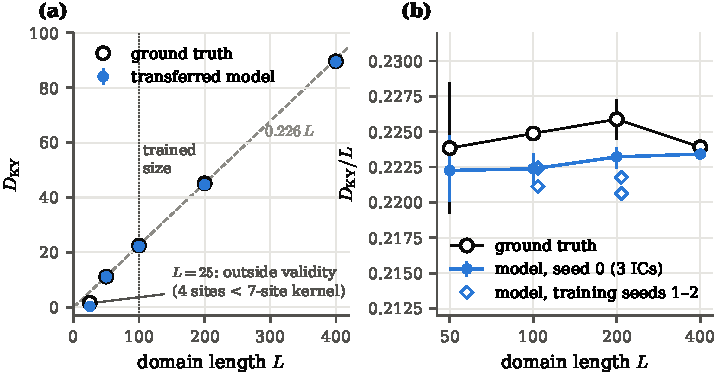
\includegraphics{figures/fig03_1d_transfer.pdf}
\caption{Zero-shot transfer of the 1D KS model trained at $L=100$.
(a) Kaplan--Yorke dimension of the PDE (open circles) and of the
transferred model (filled) against domain length; the dashed line is
$0.226L$. At $L=25$ the transferred lattice has 4 sites, fewer than one
propagator kernel spans, and the size is outside the model's domain of
validity (text). (b) Dimension per unit length for $L\ge50$, including
two independently trained models (diamonds) at $L=100$ and $L=200$; note
the vertical range, $0.2125$--$0.2325$. Bars span three initial
conditions (model) and two or three independent finite-time runs
(truth). The model sits $0.2$--$1.2\%$ below the truth at every size.}
\label{fig:transfer1d}
\end{figure*}

\begin{figure*}[htbp]
\centering
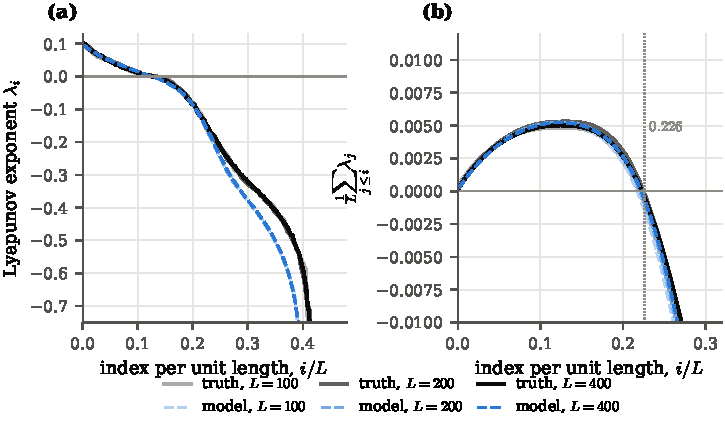
\includegraphics{figures/fig04_1d_spectra.pdf}
\caption{Lyapunov spectra of the transferred 1D model (dashed, blue) and of
the PDE (solid, gray to black) at $L=100$, $200$ and $400$; lighter lines
are smaller domains. (a) Exponents against index per unit length. (b)
Cumulative sum per unit length; it crosses zero at the Kaplan--Yorke
dimension density, marked at $0.226$. Model spectra are averaged
index-wise over three initial conditions.}
\label{fig:spectra1d}
\end{figure*}

\para{Training seeds.} Two further models trained with the same recipe
and different random seeds give $\DKY/L = 0.2224$ and $0.2211$ at $L=100$
and $0.2218$ and $0.2206$ at $L=200$, against $0.2224$ and $0.2232$ for
the first (mean over three initial conditions). The three seeds agree to
within $0.6\%$ at the trained size and $1.2\%$ after transfer, the same
order as one model's spread over initial conditions. The transfer is a
property of the recipe, not of one checkpoint.

\para{Where transfer stops.} At $L=25$ the PDE is at most marginally
chaotic: its leading exponent, $0.0013$ over 1200 time units, is barely
distinguishable from zero, and its $\DKY$ ($1.56$ or $1.82$ depending on
the number of tangent directions) is poorly determined. The transferred
model has 4 sites, fewer than the 7 that one propagator kernel spans, so
its circular convolutions wrap onto themselves
(Appendix~\ref{app:proofs}); it is non-chaotic from two of three initial
conditions and has one positive exponent ($\DKY=1.10$) from the third.
This size is outside the model's domain of validity by construction, and
we do not score it.

\para{Beyond the dimension.} The agreement is not confined to $\DKY$:
the whole positive and near-neutral part of the Lyapunov spectrum,
plotted against $i/L$, collapses onto the truth's at all three sizes,
with a mean difference of $0.002$--$0.003$ per exponent
(Fig.~\ref{fig:spectra1d}). The model departs from the truth only in the
strongly contracting directions beyond $i/L\approx0.22$, where its
exponents are more negative; these do not enter $\DKY$. Free rollouts of
the transferred model stay bounded at every size, and the largest $|u|$
over a rollout is $3.3$--$3.7$ against $3.3$--$3.5$ for the PDE
at $L=100$--$400$. Over 900 time units of free rollout, the decoded
field's energy in each of five wavenumber bands is within about $10\%$ of
the PDE's at all three sizes (Fig.~\ref{fig:rollouts}(a--c)), and the
autoencoder alone reconstructs the field to $0.01\%$ of its variance
(Appendix~\ref{app:tables}).

\para{What this does and does not show.} The 1D result is the cleanest
in the paper: the truths are converged to about one percent
(Sec.~\ref{sec:truth_uncertainty}), the evaluation covers a factor of 8
in domain size, and the result is reproduced by three training seeds.
It uses the earlier full-reach autoencoder rather than the per-patch
design of the 2D models, is trained on whole periodic domains rather
than on crops, and carries an extra penalty for spatial coherence of the
latent (Sec.~\ref{sec:canonical_recipe}). It transfers as it is, so we
did not retrain it with the 2D recipe. Section~\ref{sec:da_results} uses the same
transferred models for data assimilation at $L=200$ and $400$.

%======================================================================
\section{Two dimensions: the training distribution decides}
\label{sec:results2d}
%======================================================================

In 1D a model trained on whole periodic domains transfers. In 2D the same
approach fails, and the cause is not the architecture but the data the
model is trained on. This section shows the failure, the fix, the
canonical recipe that results, and how well the transferred models
reproduce the scaling of $\DKY$ with domain size. All errors are relative
to the references of Table~\ref{tab:truth}; for Kolmogorov flow at
$\alpha=0.05$, $1\times$, each model run is scored against the truth from
its own initial condition (Sec.~\ref{sec:truth_uncertainty}).

%----------------------------------------------------------------------
\subsection{Training on a small periodic box fails, and coupling makes it worse}
\label{sec:box_vs_window}
%----------------------------------------------------------------------

Our first 2D models were trained, like the 1D model, on whole periodic
domains: an $8\times8$-site box for both systems. Both reproduce the
dimension of their training box tolerably (2D KS: $13.7\%$ error;
Kolmogorov flow at $\alpha=0.05$: $3.7\%$). Under transfer they degrade
(Fig.~\ref{fig:box_vs_window}). The 2D KS model is $23\%$ low at $66^2$,
consistently across three initial conditions. At $\alpha=0.05$ the
Kolmogorov model is $38\%$ low at $2\times$; at $\alpha=0.1$ it is
accurate at $2\times$ ($1.9\%$) but $15\%$ low at $3\times$ and $23\%$ low at
its own size.

The propagator of these models reaches 6 sites per step on an 8-site
periodic ring, so it sees $75\%$ of its training domain and can use the
periodic wrap-around, a self-interaction that a larger domain does not
have. The local statistics of a small box also differ from the local
statistics inside a large domain wherever the flow is not exactly
extensive. A model fitted to the box therefore learns the wrong local
rule for the domain it is deployed on.

A natural response is to give the model more non-local information. We
tried three versions, each trained on the same box: the exact
Biot--Savart velocity as an additional input (D2), a learned coarse
``regional'' scale with its own mixer (D3), and a box-trained model with
the exact velocity input (C9). All three train to low loss at the box
size, and all three collapse under transfer: $\DKY$ falls to between 0
and 5 at $2\times$ and $3\times$, errors of $93$--$100\%$
(Fig.~\ref{fig:box_vs_window}(c)). Each new coupling path is trained only
on inputs from one small periodic domain and meets wavenumbers,
amplitudes and aggregation patterns at deployment that it never saw.
More expressive coupling made transfer worse, not better.

%----------------------------------------------------------------------
\subsection{Training on windows of a large domain fixes it}
\label{sec:window_fix}
%----------------------------------------------------------------------

We kept the architecture and changed only the data: one large domain
($6\times44$ per side for 2D KS, $16\times2\pi$ wide for Kolmogorov
flow), trained on crops with forced halos (Sec.~\ref{sec:crop_training}).
For 2D KS the crops are cut in both directions, so no training sample
contains a whole periodic direction. The effect is large
(Fig.~\ref{fig:box_vs_window}):
\begin{itemize}
\item 2D KS: $13.7\%\to0.9\%$ at $44^2$ and $23\%\to3.9\%$ at $66^2$.
\item Kolmogorov, $\alpha=0.05$: $37.8\%\to7.4\%$ at $2\times$, and $6.3\%$ at
  $3\times$, a size at which no box-trained model was evaluated.
\item Kolmogorov, $\alpha=0.1$: $15.1\%\to4.0\%$ at $3\times$ and
  $23.4\%\to8.6\%$ at $1\times$, but $1.9\%\to18.8\%$ at $2\times$.
\end{itemize}
The one regression, $\alpha=0.1$ at $2\times$, is the box model's
best size; the window-trained model over-predicts there by $15$--$23\%$
across initial conditions. The window-trained models never see a $2\pi$
periodic box, yet they reproduce the dimension of that box to within
about $9\%$ at both drags.

%----------------------------------------------------------------------
\subsection{The canonical recipe}
\label{sec:canonical_results}
%----------------------------------------------------------------------

Two further changes produced the recipe of Sec.~\ref{sec:canonical_recipe}.

\para{A per-patch autoencoder.} Training on crops loses a margin of
$\Renc+\Rdec$ sites at every crop edge. A per-patch autoencoder has no
reach and no margin; with more channels it loses no accuracy, at the
price of a reconstruction error about $30\%$ higher (2D KS). At
$\alpha=0.05$ and equal training data, a per-patch autoencoder with
$c=6$ gives $8.9\%$, $7.7\%$ and $3.0\%$ error at $1\times$, $2\times$ and
$3\times$ (three initial conditions), against $7.3\%$, $7.4\%$ and $6.3\%$
for the full-reach $c=3$ model; a second training seed gives $7.6\%$,
$0.2\%$ and $3.0\%$. Removing only the decoder's reach at $c=3$ gives
$5.0\%$, $9.3\%$ and $13.3\%$ (one initial condition), with the error
growing with size: three channels cannot hold a $16\times16$ patch's
chaotic content without borrowing from neighbours, six can. At equal
$c=6$, a full-reach control is worse at $1\times$ ($15.3\%$), better at
$2\times$ ($4.5\%$) and similar at $3\times$ ($4.5\%$), from one initial
condition (Fig.~\ref{fig:appendix_panels}(b)). The per-patch
design is therefore at least as accurate, needs no crop margin, and, as
Sec.~\ref{sec:da_results} shows, makes the latent observation operator
exactly local.

\para{Rollout length.} Short rollouts in training can leave the
free-running model under-constrained (Sec.~\ref{sec:fail_regimes}), and
long ones bias $\DKY$ downward (Sec.~\ref{sec:fail_mse}). The models
reported here use $\kmax=32$ for 2D KS and for Kolmogorov flow at
$\alpha=0.025$, $\kmax=16$ at $\alpha=0.1$, and the original $\kmax=12$ at
$\alpha=0.05$; at that drag a $\kmax=32$ model trained otherwise identically
(\texttt{k\_xs005\_noreg} in Appendix~\ref{app:tables}) gives
comparable errors ($6.2\%$, $5.2\%$, $7.2\%$).

\para{Selecting a model without the truth.} At $\alpha=0.1$ we trained six
variants that differ in $\kmax$ ($16$--$32$) and in the autoencoder's
regularizers (Sec.~\ref{sec:fail_mse}). Their errors against the truth
trade off between sizes, so choosing the one with the smallest error at
one size would select on the reference itself. We instead fixed a rule
before evaluating it (Appendix~\ref{app:architecture}): a variant is
eligible if its free rollouts reproduce the training data's vorticity
variance and forcing-band energy share to within $15\%$ at every size,
and among eligible variants the one with the lowest physical-space
forecast error, eight steps ahead on the held-out validation trajectory,
is selected. All six are eligible (largest deviation $6.3\%$); the
selected model's forecast error is lower than every other variant's by
at least 4.6 paired standard errors. Its errors against the truth are
$0.9\%$, $5.9\%$ and $2.6\%$ at $1\times$, $2\times$ and $3\times$; the
variant previously chosen for its $3\times$ accuracy gives $8.8\%$,
$9.9\%$ and $2.9\%$.

\para{Results.} Table~\ref{tab:transfer2d} collects the canonical
models. For 2D KS the error is $2.0\%$ at the native size and $0.6\%$ at
$66^2$, from two initial conditions each, against truths averaged over
three and two runs. At $88^2$, where we have no truth, the model gives
$\DKY=332$ and $335$, a density of $0.043$ per unit area, the same as at
$44^2$ and $66^2$ and inside the range $0.042$--$0.043$ of the truth means.
For Kolmogorov flow the errors are $1$--$9\%$ at $\alpha=0.1$ and
$\alpha=0.05$, and larger at $\alpha=0.025$
($8$--$25\%$), where the native-size result scatters strongly across
initial conditions ($\DKY$ from 13 to 27). The weakest drag is the
hardest regime; we return to it in Sec.~\ref{sec:discussion}.

\begin{table*}[htbp]
\caption{Canonical models, zero-shot. Each entry: mean $\DKY$ over
initial conditions (number in parentheses) and mean of the per-IC
relative errors against Table~\ref{tab:truth} (at $\alpha=0.05$,
$1\times$, each IC against its matched-IC truth). The $\alpha=0.1$ model
was selected without reference to any truth (Sec.~\ref{sec:canonical_results}). Kolmogorov sizes are channel widths in
units of $2\pi$; 2D KS sizes are square boxes.}
\label{tab:transfer2d}
\begin{ruledtabular}
\begin{tabular}{llccc}
system & sizes & first size (native) & second size & third size \\
\hline
\tabinput{tables/tab04_transfer2d}
\end{tabular}
\end{ruledtabular}
\end{table*}

%----------------------------------------------------------------------
\subsection{Scaling of the dimension with domain size}
\label{sec:scaling}
%----------------------------------------------------------------------

Given the uncertainty of the Kolmogorov truths
(Sec.~\ref{sec:truth_uncertainty}), the more robust comparison is the
shape of $\DKY$ as a function of domain size, shown in
Fig.~\ref{fig:scaling}.

For 2D KS the model's dimension per base box is $83.3$--$83.6$ at all
three sizes, constant to within $0.4\%$ over a factor of 4 in area; the
truth's is $82.0$ and $84.0$ at the two sizes where it exists (means over
three and two runs). The $2.5\%$ difference between them is inside the
spread of the individual runs ($80.7$--$83.6$ at $44^2$; $82.5$ and $85.6$
per box at $66^2$), so the truth is consistent with extensive scaling,
and so is the model, as Remark~\ref{rem:extensive_model} requires.

For Kolmogorov flow the model and truth densities agree at every drag to
within the spread of the truths themselves. At $\alpha=0.05$ the model's
density is $23.3$, $23.1$ and $24.5$ per box against $21.5$, $24.3$ and
$25.1$. At $\alpha=0.1$ the model's density is $16.0$, $16.3$ and $17.4$ per box
against $15.9$, $15.4$ and $17.8$ (three runs at $2\times$ and at
$3\times$), including the truth's rise at $3\times$. At $2\times$ the model also reproduces the ordering across drags,
more dimension per box at weaker drag; at $3\times$ the $\alpha=0.025$ model
($23.7$ per box) falls below the $\alpha=0.05$ model ($24.5$), while the
truth keeps rising ($27.6$ against $25.1$).

\para{Beyond the dimension.} The decoded free rollouts reproduce the
energetic scales. For the main-text $\alpha=0.1$ model the per-patch
autoencoder reconstructs the vorticity to $1.2\%$ of its variance, and
over 180 time units of free rollout the kinetic energy in the bands
around the forcing wavenumber ($2\le|\bm k|<8$) is within $10\%$ of the
truth's at every width and the vorticity's standard deviation within
$3\%$; the energy in modes longer than the native box is two to three
times the truth's at $2\times$ and $3\times$, but under $0.5\%$ of the
total. In 2D KS,
two initial conditions per size show the model's field amplitude and
large-scale energy share within the scatter between initial conditions
at every size, with no drift between the first and second halves of a
rollout. The one systematic defect is local: the per-patch decoder puts
$1.7$--$2.4\%$ of the energy at $|\bm k|\ge1.4$, against $0.5$--$0.8\%$ in
the truth, near the patch wavenumber $2\pi/h\approx1.14$
(Fig.~\ref{fig:rollouts}(d--f)). These are seams at patch edges, already present in the reconstruction of the true
field ($2.6$--$2.9\%$ error), so they come from the decoder rather than
the dynamics; they do not affect $\DKY$ and we return to them for data
assimilation in Part~II. Full tables are in Appendix~\ref{app:tables}.

%----------------------------------------------------------------------
%----------------------------------------------------------------------
\subsection{Why a model of finite reach suffices}
\label{sec:chaos_scale}
%----------------------------------------------------------------------

A local model can represent the dynamics only if the unstable directions
are themselves local. For Kolmogorov flow at $\alpha=0.05$, $3\times$, we
decomposed the unstable subspace (the span of the Lyapunov vectors with
positive exponents) by scale, for the truth and for the window-trained
full-reach $c=3$ model of Sec.~\ref{sec:window_fix} (the analysis was not
repeated for the canonical models or the other systems). The true flow
has 36 unstable directions and the model 34, with nearly identical scale content:
$9.1\%$ of the unstable-subspace variance lies at scales larger than the
$2\pi$ box in the truth and $10.0\%$ in the model. In the truth, $31.5$ of
the 36 unstable directions sit in the wavenumber band $|\bm k|\in[2,8)$
around the forcing wavenumber $k=4$, and essentially none below $|\bm k|=1$.
The chaos lives at the forcing scale, which spans a few sites, and that is
the scale a model with a reach of a few sites resolves best. The same
analysis shows no deficit of large-scale unstable directions in the
model, so we have no evidence that the remaining errors come from missing
long-range coupling.

\begin{figure*}[htbp]
\centering
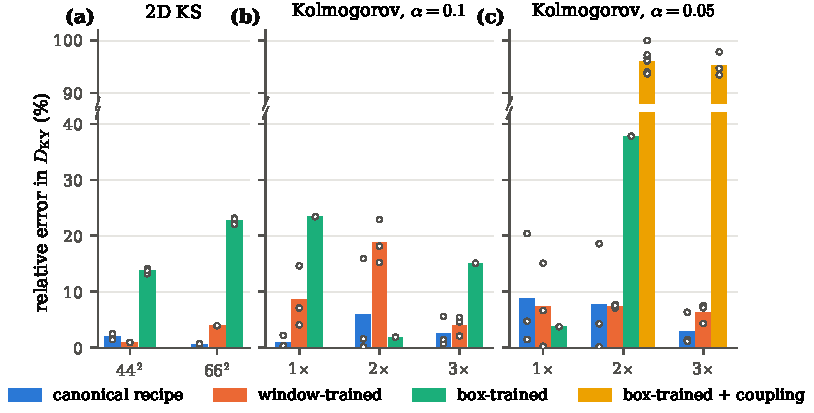
\includegraphics{figures/fig05_box_vs_window.pdf}
\caption{Relative error in $\DKY$ for four training recipes, on a linear
axis broken between $42\%$ and $88\%$; only the box-trained models with
added coupling land above the break. Bars are means over initial
conditions, dots individual initial conditions. Every window-trained and
canonical evaluation is below $25\%$, while box-trained models with
coupling miss by more than $90\%$. Box-trained: an $8\times8$-site
periodic box; with coupling: the exact Biot--Savart velocity (D2), a
learned regional scale (D3), or both box training and the exact velocity
(C9), all at $\alpha=0.05$; window-trained: the same architecture trained
on crops of a large domain; canonical: per-patch autoencoder with $c=6$
and long free rollouts. All evaluations use initial conditions
standardized with the training statistics, except the $\alpha=0.1$
box-trained $3\times$ value, for which only a raw-initial-condition
evaluation exists.}
\label{fig:box_vs_window}
\end{figure*}

\begin{figure*}[htbp]
\centering
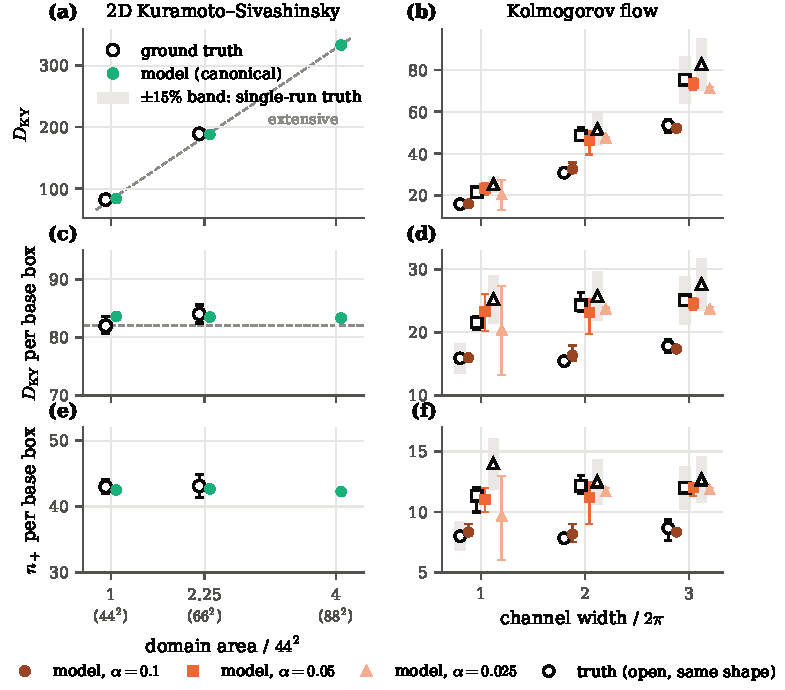
\includegraphics{figures/fig06_scaling.pdf}
\caption{Scaling of the dimension and of the number of unstable
directions with domain size. Rows: $\DKY$; $\DKY$ per base box ($44^2$
for 2D KS, $2\pi\times2\pi$ for Kolmogorov flow); number of positive
exponents $n_+$ per base box. Open markers: ground truth, with bars
spanning the runs where several exist and a shaded $\pm15\%$ band where a
size rests on one run (the run-to-run spread of Appendix~\ref{app:groundtruth});
filled markers: canonical models, with bars spanning initial
conditions. (a,c,e) 2D KS, where both sides of the box grow; the dashed
line is extensive scaling from the native truth. (b,d,f) Kolmogorov flow,
where the channel widens at fixed height; marker shape and lightness
give the drag. Both densities stay flat in 2D KS, for the truth and the
transferred model; in Kolmogorov flow the models track the truth at
$\alpha=0.1$ and $0.05$ and fall below it at $\alpha=0.025$.}
\label{fig:scaling}
\end{figure*}

\begin{figure*}[htbp]
\centering
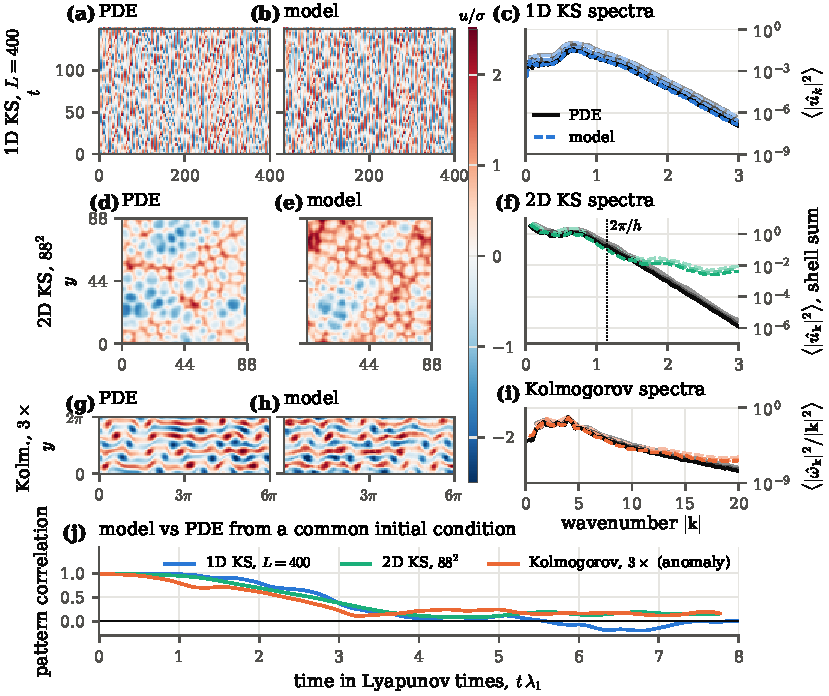
\includegraphics{figures/fig07_rollouts_spectra.pdf}
\caption{Free rollouts, energy spectra and pattern correlation after
transfer, one system per row; columns: PDE, transferred model from the
same encoded initial condition, time-averaged spectra against wavenumber
(solid: PDE; dashed: model; lighter lines: smaller domains). (a--c) 1D KS at $L=400$, four times the training size,
first 150 time units; spectra at $L=100$, $200$, $400$. (d--f) 2D KS at
$88^2$, four times the area of the base box, 35 time units after the
initial condition; spectra at $44^2$, $66^2$, $88^2$; the dotted line is
the patch wavenumber $2\pi/h$. (g--i) Kolmogorov flow at $\alpha=0.1$ and
$3\times$ (the main-text model), vorticity 40 time units after the initial
condition; kinetic-energy spectra at $1\times$, $2\times$, $3\times$.
Spectra: steps $100$--$999$ of a 1000-step rollout. (j) Spatial
correlation between model and PDE fields against time in Lyapunov times
$t\lambda_1$ (truth $\lambda_1$ at the largest size with a truth); for
Kolmogorov flow the PDE's mean vorticity profile in $y$, which is locked
to the forcing, is removed first. In all three systems the correlation
falls below $0.5$ after $2.3$--$2.9$ Lyapunov times while the spectra
stay on the PDE's: the models lose the trajectory, not the statistics.
In 2D it settles at $0.15$--$0.2$, a slowly varying large-scale component
shared over this window. The per-patch decoder leaves seams in 2D KS,
seen as excess energy beyond $2\pi/h$.}
\label{fig:rollouts}
\end{figure*}

%======================================================================
\section{Data assimilation in the local latent field}
\label{sec:da_results}
%======================================================================

Part~II asks whether the local structure that lets a model transfer
also lets a filter work on large domains with a fixed ensemble. The
models are those of Part~I, deployed at each size without retraining;
the filters run entirely in their latent space and observe the physical
field.

%----------------------------------------------------------------------
\subsection{Setting: exact locality and what is measured}
\label{sec:da_setting}
%----------------------------------------------------------------------

\para{Twin experiments.} At each domain size the truth is a trajectory of
the PDE itself, integrated at the deployment resolution from a spun-up
state. Every $5$ model steps (5 time units in 1D, $0.5$ in 2D KS, about
$0.5$ and $0.1$ Lyapunov times) we observe the field at the points of a
regular network with spacing $3.125$ (1D) or $2.75$ (2D KS) length
units, two observations per site in 1D and four in 2D, with independent
Gaussian errors of standard deviation $0.1$ in the standardized units of
the training data. The initial ensemble is the encoded initial truth
plus independent perturbations of standard deviation $0.1$ per latent
coordinate; the forecast adds model noise of standard deviation $0.08$
per coordinate at every step (Sec.~\ref{sec:da_method}). Each run has
$100$ cycles. The free run starts from the same ensemble, evolves with
the same model, receives no observations and no model noise; the error
of its ensemble mean is the reference that skill is measured against.

\para{Filters.} Section~\ref{sec:da_method} defines the three analysis
schemes. We name them by what they compute, since the literature uses
``LETKF'' for several. The \emph{dense filter} is a stochastic ensemble
Kalman filter (EnKF) with perturbed observations and Schur-product
localization of the full $\dlat\times\dlat$ forecast covariance. The
\emph{per-site filter} performs one analysis per site, in the
local-analysis form of \citet{hunt2007}, with each observation's error
variance divided by its taper value, but with the same
perturbed-observation update as the dense filter; it is therefore a
local stochastic ensemble Kalman filter rather than an ensemble
transform filter. Its deterministic counterpart, the local ensemble
transform Kalman filter of \citet{hunt2007} with the same localization,
gives the same skill to within $2\%$ at $\Nens=64$ (Appendix~\ref{app:da}) and is
reported where it differs. In 1D the analysis is also done with the
particle flow filter (PFF), and both 1D filters use the same Gaspari--Cohn
(GC) taper of half-width $3$ sites.

\para{Why the per-site filter is exact.} The decoder of the 2D models is
per-patch ($\Rdec=0$), so by Proposition~\ref{prop:blockdiag} the
Jacobian of the observations with respect to the latent field is
block-diagonal: an observation depends only on the $c$ channels of the
site whose patch contains it. Two consequences make the filter scale.
The whole Jacobian is obtained from $c=6$ forward-mode derivatives at
any domain size, and each site's analysis uses only the ensemble at the
few sites that own an observation inside its taper support, without
truncating any observation's dependence on the latent state. The local
analysis is not an approximation of a global one that happens to be
local; it is the analysis of a problem that is local. The dense filter,
by contrast, stores $\dlat\times\dlat$ matrices, whose memory grows with
the square of the area.

\para{Metrics.} The \emph{error} at an analysis time is the
root-mean-square difference, per latent coordinate, between the
ensemble-mean latent field and the encoded truth,
$\|\bar z - \E(u)\|/\sqrt{\dlat}$; the free run's error is defined the
same way. \emph{Skill} is the ratio of free-run error to analysis error:
above 1 the filter helps, below 1 it makes the estimate worse than not
assimilating at all. \emph{Spread} is the ensemble standard deviation per
coordinate, and \emph{calibration} the ratio of spread to error, which is
1 for an ensemble that represents its own uncertainty correctly and
below 1 for an over-confident one. All reported values are
\emph{steady-state} averages over cycles $51$--$100$, after the initial
transient. Because the latent coordinates are learned, we also measure
the error in physical space: the root-mean-square difference between
the decoded ensemble mean and the true field, at every grid point and at
the observed points separately, against the floor set by the decoder
alone, $\|\Dec(\E(u))-u\|$.

\para{How large an ensemble the problem demands.} Without localization a
filter needs at least as many members as there are unstable and neutral
directions \citep{bocquetcarrassi2017}; for a deterministic filter on
Lorenz-96 the minimum is $n_+ + 1$, with $n_+$ the number of positive
Lyapunov exponents \citep{takeda2026}. These counts are measured here.
For 2D KS the truth has $n_+ = 42$--$44$ at $44^2$ and $93$--$101$ at $66^2$,
and the transferred model has $n_+ = 168$--$170$ at $88^2$ (Table~\ref{tab:truth}
and Appendix~\ref{app:tables}); for 1D KS the truth has $n_+ = 26$--$27$ at
$L=200$ and $50$--$51$ at $L=400$ (Appendix~\ref{app:truth_list}). A fixed ensemble of 64 members is therefore above
this bound only at the native 2D size and at $L=200$ in 1D. An
unlocalized filter of that size should fail beyond them; a localized
filter needs only to span the unstable directions inside its taper
support, Eq.~\eqref{eq:nens_local}, which do not grow with the domain.
The following sections test both predictions.

%----------------------------------------------------------------------
\subsection{A fixed ensemble across a hundredfold area}
\label{sec:da_2d}
%----------------------------------------------------------------------

Table~\ref{tab:da_2d_sizes} and Fig.~\ref{fig:da_2d} give the central result of Part~II. The 2D KS
model, trained on windows of a $264^2$ simulation, is deployed on square
domains from $44^2$ to $440^2$, a factor of 100 in area and in latent
dimension ($\dlat=384$ to $38\,400$), and the same per-site filter with 64
members assimilates the same observation network at every size. Its
steady-state skill is $4.23$ at $44^2$ and $3.84$--$4.08$ at every larger size,
$3.90$ at $440^2$: the filter loses less than $10\%$ of its skill over the
whole range. A second seed at every size from $44^2$ to $330^2$ changes the
skill by at most $0.15$.

An unlocalized filter with the same 64 members does what the bound of
Sec.~\ref{sec:da_setting} predicts. At $44^2$, where $64$ exceeds the
$42$--$44$ unstable directions, it helps (skill $2.31$); at $66^2$, with
$93$--$101$, and at $88^2$, with about 170, it is worse than no
assimilation ($0.94$ and $0.83$). Doubling the ensemble to 128 restores
skill where 128 exceeds $n_+$ ($3.47$ at $44^2$, $2.22$ at $66^2$) and not where
it does not ($1.11$ at $88^2$). The dense filter with Gaspari--Cohn
localization, which applies the same taper to the full covariance,
works at every size it can be run at ($3.40$--$3.65$), $11$--$14\%$ below the
per-site filter, but its memory grows with the square of the area
(Sec.~\ref{sec:da_cost}), and beyond $220^2$ we did not run it.

\para{Ensemble size.} Table~\ref{tab:da_2d_ensemble} shows the per-site
filter's skill against ensemble size. It is the same at every domain
size: about $1.1$ with 8 members, $1.8$--$2.1$ with 16, $3.3$--$3.8$ with 32,
$3.8$--$4.2$ with 64 and slightly lower again with 128. That the required
ensemble does not depend on the domain size is the point. The level it
settles at is set by the local problem: Eq.~\eqref{eq:nens_local} with
the 2D KS density of $0.043$ per unit area and the taper's support (radius
$33$ length units) gives an estimate of about 150, far above the 32--64
members that suffice, so the heuristic is conservative here, as one
expects when the errors inside the support are dominated by a few
unstable directions. The dense filter with localization already reaches
$3.5$--$3.8$ with 16 members, where the per-site filter does not. The
deterministic transform behaves like the perturbed-observation update
at every ensemble size ($1.87$ at 16 members), so observation sampling
noise is not the cause. The likely cause is the localization form: the
dense filter tapers the covariance itself, while the per-site filter
tapers only the observation errors and uses the untapered sample
covariance among the sites inside its support, which 16 members estimate
poorly. We have not tested this.

\para{Calibration and model noise.} The ensemble is over-confident:
its spread is about a third of its error at every size ($0.33$--$0.37$ for
the per-site filter, $0.40$--$0.43$ for the dense one). Inflating the
forecast perturbations by up to $20\%$ changes neither skill nor
calibration by more than $9\%$ (Appendix~\ref{app:da}): with four observations per
site, the analysis is set by the observations rather than by the prior
spread. The model noise is the effective control. Halving it from $0.08$ to
$0.04$ raises the skill by $13$--$14\%$ and lowers the calibration by $0.03$, by
the same amounts at $44^2$, $88^2$ and $220^2$ (skill $4.79$, $4.55$, $4.33$), so this
trade-off, too, does not depend on the domain size.

\para{In physical space.} The latent error is measured against the
encoded truth, so it cannot see what the decoder loses. Decoding the
analysis mean, its root-mean-square error against the true field in
steady state is $1.05$, $0.99$, $1.01$ and $1.02$ at $44^2$, $88^2$, $220^2$ and
$330^2$, and $0.79$--$0.82$ at the observed points (observation error $0.62$
in these units), against a floor of $0.65$--$0.69$ for the decoder alone,
$\|\Dec(\E(u))-u\|$. The analysis error does not depend on the domain
size, and about $40\%$ of its variance is the decoder's. (The field's
standard deviation grows from $4.0$ at $44^2$ to $9.1$ at $330^2$ as larger
domains hold more large-scale variability, so the error relative to the
field shrinks with size.) In physical space the skill is $4.5$--$6.2$,
against $3.8$--$4.2$ in latent space. The decoder's error sits mostly at
patch edges: at every size from $44^2$ to $330^2$ the mean gradient across a
patch edge is $3.6$ times that inside a patch in the reconstruction of
the true field, $3.8$ times in the analysis and $3.0$ in the free run,
against $1.0$ in the truth. These are the seams of Sec.~\ref{sec:scaling},
set by the decoder and barely changed by the assimilation
(Fig.~\ref{fig:da_snapshot}).

\begin{figure*}[htbp]
\centering
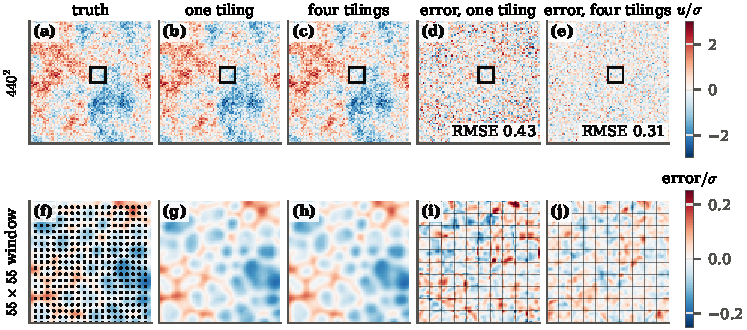
\includegraphics{figures/fig11_da_snapshot.pdf}
\caption{One steady-state analysis at $330^2$ ($\dlat=21\,600$, 64 members,
cycle 78 of 100), fields divided by the training standard deviation.
Top: the whole domain; the square marks the $55\times55$ window shown
below. (a, e) Truth, with the observation sites in the window; (b, f)
free run, the mean of the 64 unassimilated members, which have
decorrelated from the truth and from each other, so their mean keeps
only the large-scale pattern; (c, g) analysis, the decoded ensemble
mean; (d, h) analysis error, with patch edges drawn in the window.
Root-mean-square errors in field units. The analysis recovers the
cellular pattern everywhere; much of its residual error is small-scale
and largest at patch edges.}
\label{fig:da_snapshot}
\end{figure*}

\begin{figure*}[htbp]
\centering
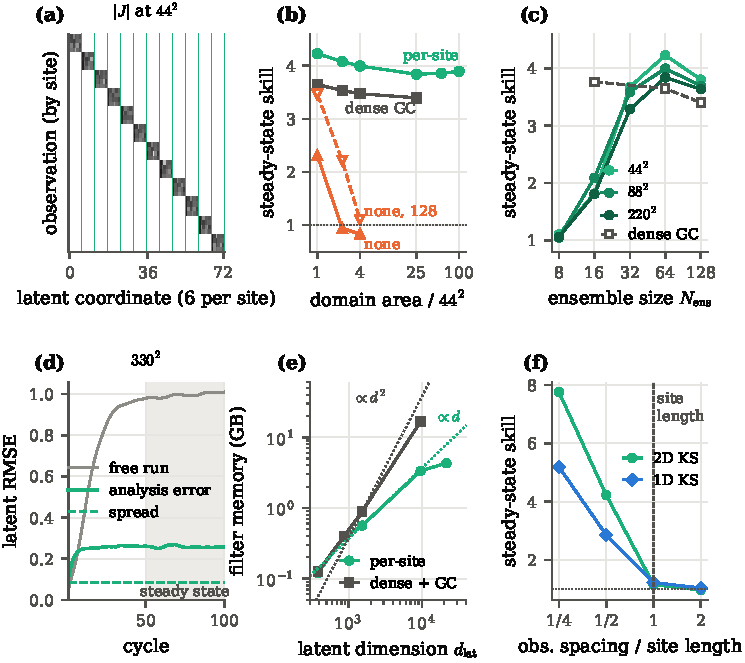
\includegraphics{figures/fig09_2d_da.pdf}
\caption{Data assimilation in the 2D KS latent field. (a) Magnitude of
the observation Jacobian at $44^2$, computed densely by reverse-mode
differentiation, with observations sorted by the site that owns them
(12 of the 64 sites): it is exactly zero outside the six columns of each
site (largest off-block entry $0$, largest entry $1.6$), as
Proposition~\ref{prop:blockdiag} states. (b) Steady-state skill against
domain area with 64 members (and 128 for the unlocalized filter): the
per-site filter keeps its skill over a hundredfold area; the
unlocalized filter fails where the truth's $n_+$ ($42$--$44$ at $44^2$,
$93$--$101$ at $66^2$) exceeds the ensemble. (c) Skill against ensemble size
for the per-site filter at three sizes, and for the dense filter with
Gaspari--Cohn localization at $44^2$. (d) Per-cycle analysis error,
spread and free-run error at $330^2$ ($\dlat=21\,600$); shaded: the
steady-state window. (e) Peak memory of the filter alone against latent
dimension, with guides proportional to $\dlat$ and $\dlat^2$ through the
$88^2$ points; from $220^2$ to $330^2$ the per-site filter's memory grows less
than linearly. (f) Skill against observation spacing in units of the
site length, for 2D KS at $44^2$ and 1D KS at $L=200$: assimilation fails once the spacing
reaches the site length in both systems.}
\label{fig:da_2d}
\end{figure*}

\begin{table*}[htbp]
\caption{2D KS data assimilation across domain sizes, steady-state
skill (calibration in parentheses), observation spacing $2.75$, 100
cycles. $n_+$: positive Lyapunov exponents of the truth; $^a$of the
transferred model, no truth at this size. Per-site: the per-site filter
with 64 members, seed 0 and, after the comma, seed 1. Dense GC: dense
filter with Gaspari--Cohn localization, 64 members. Unlocalized: dense
filter without localization, 64 and 128 members. ---: not run (the dense
filter's memory grows with the square of the area).}
\label{tab:da_2d_sizes}
\widetabular{lcccccc}{
size & $\dlat$ & $n_+$ & per-site, 64 & dense GC, 64 & unlocalized, 64 & unlocalized, 128 \\
\hline
\tabinput{tables/tab07_2d_sizes}}
\end{table*}

\begin{table*}[htbp]
\caption{Steady-state skill against ensemble size, 2D KS. Per-site
filter (perturbed observations) at four domain sizes; its deterministic
transform variant at $44^2$; dense filter with Gaspari--Cohn localization
at three sizes. ---: not run.}
\label{tab:da_2d_ensemble}
\widetabular{ccccccccc}{
$\Nens$ & per-site $44^2$ & $66^2$ & $88^2$ & $220^2$ & transform $44^2$ & dense GC $44^2$ & $66^2$ & $88^2$ \\
\hline
\tabinput{tables/tab07_2d_ensemble}}
\end{table*}

%----------------------------------------------------------------------
\subsection{Observation density and the one-dimensional results}
\label{sec:da_1d}
%----------------------------------------------------------------------

\para{How dense the network must be.} In both systems the filter needs
observations inside every patch. With the per-site filter at $44^2$ and
$\Nens=64$, the steady-state skill is $7.8$ at an observation spacing of
$1.4$ length units, $4.2$ at $2.75$, and $1.2$ and $1.0$ at $5.5$ and $11$. In
1D at $L=200$ with the particle flow filter and Gaspari--Cohn
localization it is $5.2$, $2.9$, $1.2$ and $1.0$ at spacings $1.6$, $3.1$,
$6.25$ and $12.5$. Assimilation fails once the spacing reaches the site
length ($5.5$ in 2D, $6.25$ in 1D), well below the pattern wavelength
$2\sqrt2\,\pi\approx8.9$: a site whose patch holds no observation is
corrected only through its neighbours' covariances, which the latent
field carries poorly. All other runs use half the site length.

\para{1D after transfer.} Table~\ref{tab:da_1d} and Fig.~\ref{fig:da_1d} give the 1D results at
$L=200$ and $400$, two and four times the training size, at a fixed
observation spacing of $3.125$. With localization, skill is $2.3$--$3.0$ for
every ensemble of 16 or more members, at both sizes and with both
filters. Without localization the filter makes the estimate worse than
no assimilation (skill below 1) until the ensemble is large enough, and
how large depends on the domain: at $L=200$, where $n_+=26$--$27$, it is marginal
at 64 members ($1.1$--$1.3$) and works at 128 ($2.5$--$2.7$); at $L=400$, where
$n_+=50$--$51$, it fails at 64 ($0.8$), is marginal at 128 ($1.2$--$1.4$) and
works only at 256 ($2.5$--$2.7$). The number of members an unlocalized
filter needs doubles with the domain, as the bound of
Sec.~\ref{sec:da_setting} predicts, while the localized filter needs
the same 16 at both sizes. The particle flow filter and the ensemble
Kalman filter differ by at most $0.4$ in skill and show the same pattern
at every point, so the result does not depend on the analysis scheme.

An earlier version of this experiment scaled the observation stride
with the domain, which doubled the observation spacing with every
doubling of $L$, to $6.25$ at $L=200$ and $12.5$ at $L=400$. At those spacings
the localized filter's skill at $L=200$ was about $1.3$, against $2.9$ at
the fixed spacing used here.

\para{Distance-free localization.} Sampling error correction
\citep{anderson2012} needs no distance, and is therefore the natural
competitor of a latent field that has one. At the training size, in an
earlier comparison with 40 cycles, SEC applied to a global latent vector
beat Gaspari--Cohn applied to the local field at every ensemble size,
with analysis errors $5$--$25\%$ lower. That comparison confounds the
localization with the architecture (two different autoencoders), and at
$L=100$ the taper is non-zero on 11 of the 16 sites of the ring, so it
hardly localizes. At the transfer size the comparison can be made
on one latent. The SEC-corrected covariance, formed elementwise, is
indefinite at five of six ensemble sizes, and the particle flow filter,
which factorizes it, fails. This is a property of the matrix form, not of
SEC: projecting the corrected matrix onto the positive semidefinite cone,
or applying the correction to each regression coefficient in a serial
filter, the form \citet{anderson2012} uses, both run at every ensemble
size. Gaspari--Cohn beats both at every size below 256 members: by a
factor of up to $1.7$ against the projected form (both with the particle
flow filter) and up to $3.5$ against the serial form (both ensemble
Kalman filters), and the serial form does not help at all below 128
members (Table~\ref{tab:da_1d}). SEC removes
sampling noise from correlations; a distance taper also removes the many
weak true correlations between distant sites, and that is what the small
ensemble cannot afford to estimate.

\begin{figure*}[htbp]
\centering
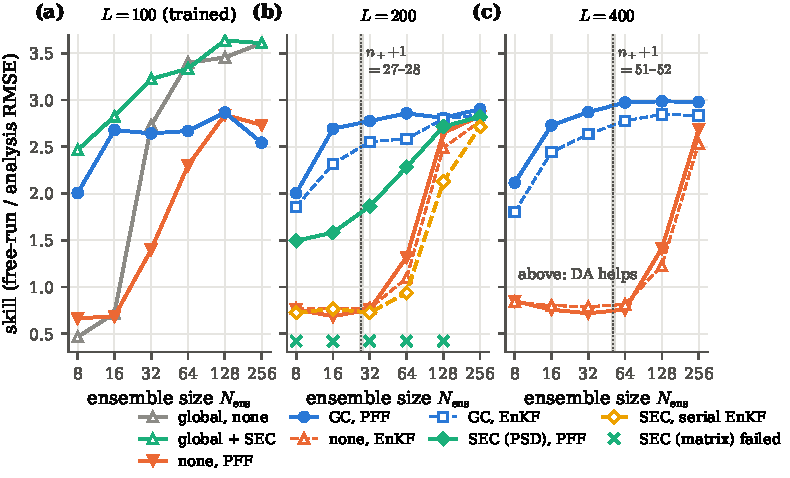
\includegraphics{figures/fig08_1d_da.pdf}
\caption{1D KS data assimilation: skill (free-run error over analysis
error; above the dotted line assimilation helps) against ensemble size,
observation spacing $3.125$ in every panel. (a) Training size $L=100$
(earlier sweeps, 40 cycles, whole-run skill): a global latent vector
without localization and with sampling error correction (SEC), and the
local field without localization and with Gaspari--Cohn (GC), particle
flow filter, drawn with the symbols of the particle-flow curves in (b,c). (b) $L=200$ and (c) $L=400$, the local model transferred
without retraining (100 cycles, steady state): no localization and GC,
for the particle flow filter (solid) and the ensemble Kalman filter
(dashed); in (b) also SEC after projection onto the PSD cone and in a
serial filter, with crosses at the ensemble sizes where SEC in matrix
form failed. The shaded line marks $n_++1$ for the truth. With
localization a 16-member ensemble suffices at both sizes; without it,
the ensemble must exceed the number of unstable directions by a margin,
and that number doubles with the domain.}
\label{fig:da_1d}
\end{figure*}

\begin{table*}[htbp]
\caption{1D KS data assimilation after transfer: steady-state skill
(free-run error over analysis error, cycles 51--100) at a fixed
observation spacing of $3.125$, model trained at $L=100$. Pairs: no
localization / Gaspari--Cohn (half-width 3 sites). Last two columns
($L=200$ only): sampling error correction with the particle flow filter
after projection onto the PSD cone, and in a serial ensemble Kalman
filter. Skill below 1 means the filter is worse than no assimilation.}
\label{tab:da_1d}
\widetabular{ccccccc}{
$\Nens$ & PFF, $L=200$ & PFF, $L=400$ & EnKF, $L=200$ & EnKF, $L=400$ & SEC-PSD & serial SEC \\
\hline
\tabinput{tables/tab07_1d_da}}
\end{table*}
%----------------------------------------------------------------------
\subsection{Cost and memory}
\label{sec:da_cost}
%----------------------------------------------------------------------

Table~\ref{tab:da_cost} gives what the filters cost. Memory is the peak
resident memory of the filter alone, measured as the peak over a run
minus the peak once the truth has been generated. The per-site filter
needs $0.12$, $0.39$, $0.56$, $3.35$ and $4.30$~GB at $\dlat=384$, $864$, $1536$,
$9600$ and $21\,600$. From $88^2$ to $220^2$ the latent dimension grows
$6.25$-fold and the memory $5.96$-fold, and from $220^2$ to $330^2$ the
dimension grows $2.25$-fold and the memory $1.28$-fold: the filter's memory
grows no faster than the domain area, as Proposition~\ref{prop:blockdiag}
implies. The dense filter needs the
same at the native size but $16.75$~GB at $220^2$, about 24 copies of one
$\dlat\times\dlat$ matrix; at $330^2$ a single such matrix is $3.5$~GB and at
$440^2$ it is $11$~GB, so we did not run it there.

Time is less favourable to the per-site filter at small sizes. Over a
whole run, including the integration of the PDE truth, the per-site
filter takes two to four times the dense filter's CPU time up to $88^2$,
because it loops over sites in Python while the dense filter performs a
few large matrix products. The two cross between $88^2$ and $220^2$
($1450$ against $1914$~s at $220^2$), and from there the per-site filter's
time grows in proportion to the area ($\times4.4$ from $220^2$ to $440^2$
for $\times4$ in area). The deterministic variant is about $40\%$ faster
than the perturbed-observation one, having no observation draws. The
CPU times carry run-to-run noise of tens of percent from other jobs on
the same machine (the $66^2$ point is slower than the $88^2$ one); we
have not profiled the per-site loop, which is the obvious target for a
vectorized implementation. The observation Jacobian itself is cheap:
its six forward passes take $1.3$~ms at $44^2$ and $49$~ms at $440^2$, where
dense reverse mode would need one pass per observation
(Appendix~\ref{app:da_jacobian}).

\begin{table}[htbp]
\caption{Cost of the per-site and dense filters, 2D KS, $\Nens=64$, 100
cycles. $\dlat$: latent dimension; filter memory: peak resident memory
minus the peak after the truth is generated (GB); $\dlat^2$: memory of one
dense $\dlat\times\dlat$ matrix in double precision (GB); CPU: whole-run
user plus system time, including the PDE truth (s). ---: not run, or no
clean memory measurement yet.}
\label{tab:da_cost}
\begin{ruledtabular}
\begin{tabular}{lcccccc}
size & $\dlat$ & \multicolumn{2}{c}{filter memory} & $\dlat^2$ & \multicolumn{2}{c}{CPU} \\
 & & per-site & dense & & per-site & dense \\
\hline
\tabinput{tables/tab_da_cost}
\end{tabular}
\end{ruledtabular}
\end{table}

%======================================================================
\section{What does not work, and why}
\label{sec:failure}
%======================================================================

The recipe of Sec.~\ref{sec:canonical_recipe} is the end point of many
attempts. We report the four failures that bear on the claims above.
Errors are means of per-IC relative errors over three initial conditions
against the truths of Table~\ref{tab:truth} unless stated; every number
is in Appendix~\ref{app:tables}.

%----------------------------------------------------------------------
\subsection{Softmax attention}
\label{sec:fail_attention}
%----------------------------------------------------------------------

In 1D, every propagator that mixed sites by self-attention, windowed or
global, collapsed to a fixed point under free rollout ($\DKY=0$) while its
short-horizon validation loss was competitive. Replacing the attention
by the linear mixer of Eq.~\eqref{eq:mixer_block}, at the same radius,
removed the collapse. In 2D we replaced only the encoder's site mixing by
windowed attention with a relative position bias, which keeps exact
equivariance, on a box-trained Kolmogorov model at $\alpha=0.1$. Its
Stage~B validation loss was three times lower than the convolutional
encoder's, yet from one initial condition its $\DKY$ was $30\%$ low at both
$1\times$ and $2\times$, against $20\%$ and $3\%$ for the convolutional
model.\footnote{Both from unstandardized initial conditions, the only
evaluation available for these two models.} A more flexible mixer fits
the training domain more closely and transfers worse, and short-horizon
losses predicted neither failure.

%----------------------------------------------------------------------
\subsection{Coupling and context do not replace the right data}
\label{sec:fail_coupling}
%----------------------------------------------------------------------

Adding non-local inputs to a box-trained model makes transfer worse
(Sec.~\ref{sec:box_vs_window}); with window training the same additions
are merely unhelpful. At $\alpha=0.05$ the window-trained model has errors
of $7.3\%$, $7.4\%$ and $6.3\%$ at $1\times$, $2\times$ and $3\times$. A learned
consensus mechanism that exchanges messages between sites gives $7.0\%$,
$6.7\%$ and $9.2\%$; the exact Biot--Savart velocity as an extra input gives
$9.4\%$, $8.2\%$ and $11.4\%$. Doubling the number of independent training
trajectories from four to eight changes the canonical-recipe errors from
$6.2\%$, $5.2\%$, $7.2\%$ to $5.5\%$, $4.4\%$, $9.6\%$, so the amount of data is
not what limits accuracy at $3\times$ either.

%----------------------------------------------------------------------
\subsection{Short rollouts allow spurious regimes}
\label{sec:fail_regimes}
%----------------------------------------------------------------------

A Kolmogorov model trained on $40\times40$-site crops with rollouts of at
most 12 steps has low validation losses, but its free rollouts leave the
attractor. On the native box its vorticity standard deviation is $0.98$
against the truth's $1.40$, and half of its kinetic energy sits at
$|\bm k|<2$ against $10\%$ in the truth; at $3\times$ it settles into a
different, more energetic state, and its $\DKY$ there ranges from $65$ to
$107$ across three initial conditions (Fig.~\ref{fig:failure}(c)). The
true flow shows no such regimes over 400 time units. Retraining the
propagator with rollouts up to $\kmax=32$ removes them: variance and
forcing-band energy share return to within $5\%$ of the truth's at every
size, and the spread of $\DKY$ at $3\times$ falls from $51\%$ to $5\%$. The
cost is the bias of the next subsection: the retrained model, which
also raised the terminal input noise from $0.02$ to $0.05$, is $4\%$, $13\%$
and $14\%$ low at the three widths (Remark~\ref{rem:noise_penalty}).
Free-rollout statistics need no truth and catch this failure before
any Lyapunov computation, which is why they screen every model
(Sec.~\ref{sec:evaluation}).

%----------------------------------------------------------------------
\subsection{Squared-error rollouts damp the dimension}
\label{sec:fail_mse}
%----------------------------------------------------------------------

Lemma~\ref{lem:mse} predicts that longer squared-error rollouts bias
$\DKY$ down, and where models differ in $\kmax$ and little else this is
what happens (Fig.~\ref{fig:failure}(b)). Raising $\kmax$ from 12 to 32
lowers $\DKY$ at every size, by $0.4$--$6$ points of relative error for the
per-patch model at $\alpha=0.05$ and by $17$--$25$ points for the 2D-crop
model above; raising it from 16 to 32 at $\alpha=0.1$ lowers it by $3$--$10$
points. The bias is not a loss of amplitude: started from the validation
trajectory, every model we checked ($\kmax$ from 12 to 32, both drags)
keeps its vorticity variance within $2.3\%$ of the truth's at every lead
up to 64 steps. The contraction acts on the growth of perturbations,
which is what $\lambda_1$ and $\DKY$ measure.

Table~\ref{tab:alpha01_ablation} and Fig.~\ref{fig:failure}(a) list the
six variants trained at $\alpha=0.1$. Shortening the rollout from
$\kmax=32$ to $16$ cuts the underestimate at $3\times$ from $10.9\%$ to
$2.6\%$ (v1 to v2, with a slightly stronger barrier), and both $\kmax=20$
variants are $7$--$10\%$ low there. The offset $\epsilon$ of the log-det
barrier, which sets how hard the barrier pushes on the weakest latent
directions, is a second lever: at $\kmax=16$, setting $\epsilon=0$ moves the
$3\times$ error from $2.9\%$ to $4.9\%$ and the $1\times$ error from $8.8\%$ to
$2.8\%$ (v5 to v6). No variant is best at every size, and the size at
which a variant is most accurate is not predictable from its training
loss; that is why the main-text model was chosen by the truth-free rule
of Sec.~\ref{sec:canonical_results}. The rule also proved robust where
a truth-based choice would not have been: against the earlier single
40-unit truth at $3\times$, v5 was the most accurate variant and v2 the
second; against the three-run mean, v2 is the most accurate
(Appendix~\ref{app:groundtruth}). Two further regularizers do not help.
Without the variance term ($\wvar=0$) encoder and decoder rescale against
each other and the latent variance grows by six orders of magnitude at
constant reconstruction error. A spectral regularizer that matches the
rollout's energy shares to the training data's tightens the native-size
scatter at $\alpha=0.05$ ($5\%$ instead of $22\%$) but worsens the $3\times$
error ($9.9\%$ instead of $7.2\%$): it constrains the energy distribution,
not the growth rates that set $\DKY$.

\begin{table}[htbp]
\caption{Training variants at $\alpha=0.1$. $\epsilon$: offset of the
log-det barrier; $w_{\mathrm{var}}/w_{\mathrm{ld}}$: Stage~A regularizer
weights; val.: normalized forecast error at lead 8 on the validation
trajectory; dev.: largest deviation of the free-rollout statistics from
the training data (\%), both from the truth-free selection rule; last
three columns: error in $\DKY$ (\%) at $1\times$, $2\times$, $3\times$.
$^\star$Selected main-text model. $^\dagger$Trained with an additional
one-sided log-det floor on the rollout that never activated (a control
without it is identical to machine precision).}
\label{tab:alpha01_ablation}
\begin{ruledtabular}
\begin{tabular}{lcccccccc}
variant & $\kmax$ & $\epsilon$ & $w_{\mathrm{var}}/w_{\mathrm{ld}}$ & val. & dev. & $1\times$ & $2\times$ & $3\times$ \\
\hline
\tabinput{tables/tab08_alpha01_ablation}
\end{tabular}
\end{ruledtabular}
\end{table}

\begin{figure*}[htbp]
\centering
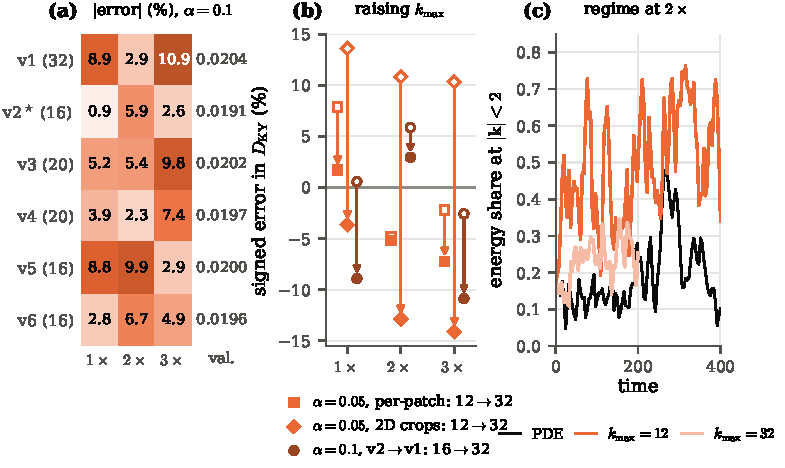
\includegraphics{figures/fig10_failure.pdf}
\caption{Failure modes in Kolmogorov flow. (a) The six training variants
at $\alpha=0.1$ (Table~\ref{tab:alpha01_ablation}): error in $\DKY$ (\%,
mean over three initial conditions) at each channel width, with
$\kmax$ in parentheses and the truth-free validation forecast error at
lead 8 in the right column; $^\star$ the selected model. No row is
lightest in every column. (b) Signed error in $\DKY$ for three pairs of models that differ in
the length of their training rollouts, short (open) to long (filled):
per-patch models at $\alpha=0.05$ ($\kmax$ 12 to 32, otherwise identical
except for training length), 2D-crop models at $\alpha=0.05$ (12 to 32,
with terminal input noise 0.05), and v2 to v1 at $\alpha=0.1$ (16 to 32).
Longer rollouts lower $\DKY$ at every size (Lemma~\ref{lem:mse}). (c)
Share of kinetic energy at $|\bm k|<2$ during free rollouts at $2\times$
from one initial condition: the PDE, the 2D-crop model trained with
$\kmax=12$, which settles into a spurious large-scale regime, and its
$\kmax=32$ retrain (rollout of 200 time units).}
\label{fig:failure}
\end{figure*}

%======================================================================
\section{Discussion and limitations}
\label{sec:discussion}
%======================================================================

\para{What transfer requires.} Four conditions emerged, and each was
necessary in at least one system. First, the physics must be extensive
at the scales involved. This can be checked before any model is trained,
from ground truth at two sizes: the 2D KS density is $82.0$ and $84.0$ per
base box at $44^2$ and $66^2$, constant within the spread of the truth runs,
while in Kolmogorov flow the truth's density per box rises with the
channel width at every drag ($15.9$, $15.4$, $17.8$ at $\alpha=0.1$; $21.5$, $24.3$,
$25.1$ at $\alpha=0.05$; $25.2$, $25.8$, $27.6$ at $\alpha=0.025$). A local model is
extensive by construction (Remark~\ref{rem:extensive_model}), so wherever
the truth is not, a transfer error is expected and is not a failure of
training. Second, the training data must contain the local statistics of
a large domain. The same architecture trained on a small periodic box
misses $\DKY$ by $15$--$38\%$ in three of the four larger configurations we
evaluated (it happens to be accurate at $\alpha=0.1$, $2\times$), and trained on
windows of one large simulation it transfers (Sec.~\ref{sec:box_vs_window}); the window
training is a limited-area problem, and Proposition~\ref{prop:halo} shows
that the forced halo trains exactly that problem. Third, the learned map
must remain chaotic, and chaotic at the right rate, when it runs freely.
Short rollouts leave room for spurious regimes
(Sec.~\ref{sec:fail_regimes}); long squared-error rollouts damp the growth
rates (Sec.~\ref{sec:fail_mse}); free-rollout statistics compared with the
training data detect the first problem without any truth, and the
truth-free selection rule of Sec.~\ref{sec:canonical_results} chose a
model that is within $0.9$--$5.9\%$ of the truth at every width. Fourth, the
model's reach must cover the interaction range of the dynamics.

\para{The interaction range is the design length.} The light cone set by
the speed at which perturbations spread is far too short to constrain the
reach of a model at these time steps (Sec.~\ref{sec:receptive}). The length
that matters is the distance beyond which neighbouring values stop
improving a one-step prediction: three to four sites, $19$--$25$ length
units, for the 1D latent dynamics, against a trained reach of six. In
Kolmogorov flow most of the unstable directions lie in the band around
the forcing wavenumber, $31.5$ of $36$ at $|\bm k|\in[2,8)$ for $\alpha=0.05$ at
$3\times$, whose wavelengths span one to four sites. Models whose encoder
reaches two sites and whose propagator reaches one fail even when trained
on windows of the very domain they are evaluated on, with errors of
$66$--$100\%$ in $\DKY$ (Appendix~\ref{app:tables}). The rule we take from this
is to measure the interaction range on data, for example by fitting a
shared stencil of increasing width, and to give the encoder and
propagator a reach that covers it with a margin. The reach then sets the
smallest domain the model can be used on, which is what fails at $L=25$.

\para{The parameters describe the law, not the state.} Because every
operator is shared by all sites, the trained parameters encode one local
rule, and their number is fixed by that rule rather than by the domain.
The 2D models have about $135{,}000$ parameters. At $66^2$ such a model
reproduces a Kaplan--Yorke dimension of $188$ to within $0.6\%$ of the truth
(Table~\ref{tab:transfer2d}), and extrapolating the measured density of
$0.043$ per unit area, the attractor at $440^2$, on which the same model is used
for data assimilation in Part~II, has a dimension of roughly $8{,}000$. A
model whose size is set by the state would have to grow with that number;
this one does not. The same weight sharing makes training cheap in data:
every window, and every site within it, is a training example of the same
rule, and the 2D KS models are trained on five trajectories of $25$ time
units. Neither a small absolute parameter count nor size independence is
new by itself: convolutional surrogates and neural operators share weights
too \citep{barsinai2019,kochkov2021}. What the dimension comparison adds is
evidence that the shared rule is the right one, in the sense that its
extension to a larger domain carries the right density of chaos. This is
the inductive bias that extensive chaos calls for: a system made of many
copies of one local process is described most economically by learning
that process once.

\para{Transfer error as a probe of the physics.} Because a local model
is extensive by construction, the difference between its dimension
density and the truth's on a larger domain measures how far the truth is
from extensive at that size, once the model is accurate at the native
size. The weakest drag, where the native-size models scatter most and the
transferred models fall below a rising truth, is where the inverse
cascade is least arrested, and we expect non-local effects to be largest
there. Using
transfer error to locate the scales at which a system stops being
extensive is a question in its own right, which we leave to future work.

\para{What locality buys in data assimilation.} The latent field makes
localization possible in a learned space, and with a per-patch decoder it
makes it exact (Proposition~\ref{prop:blockdiag}). The ensemble a localized
filter needs is then set by the local problem, about 32 members per tiling
at every size, while an unlocalized filter needs more members than the
attractor has unstable directions, a number that grows with the domain
(Secs.~\ref{sec:da_2d} and \ref{sec:da_1d}). The price of exact locality is
an error tied to the patch lattice, which the decoder does not remove; the
shifted tilings remove most of it, because the tilings' errors are only
weakly correlated, and they do so without retraining. The remaining
analysis error is mostly the filter's, not the decoder's: the blended
decoder floor is less than half of it (Sec.~\ref{sec:da_accuracy}). Better
use of the ensemble inside each tiling, and models of the propagator's
error in place of isotropic noise, are the natural next steps.

\para{When to prefer a learned model.} A filter built on the correct
equations is four times more accurate than the latent filter, and one built
on equations with a small or correctable error is still better. The
comparison of Sec.~\ref{sec:da_model_error} locates the boundary: what
matters is the part of the physical model's one-cycle forecast error that
bias correction cannot remove, and the latent filter wins once it exceeds
about a sixth of the observation error. Two features of the comparison
carry over to real systems. The errors that parameter estimation and bias
correction cannot reach are the structural ones, a wrong form of an
operator or a process that is missing or unobserved, and those are the
errors of the models of convection and cloud processes that motivate this
work. And the learned model needs no tuning for the error of the model it
replaces: one setting served every case, while the physics-based filter
worked only in a narrow window of its inflation. The model learned from
noisy fields was slightly better than one learned from clean fields, so
measurement error, the part of the error budget that is usually known, can
be handled in training. A process with memory that the current field does
not reveal limits both filters (Sec.~\ref{sec:da_model_error}); propagators
with access to past states are the obvious remedy on the learned side.

\para{Limitations.} We state them plainly.
\begin{itemize}
\item \emph{Ground truth.} The Kolmogorov truths at $\alpha=0.1$, $1\times$, at
  $\alpha=0.05$, $3\times$, and at all three widths for $\alpha=0.025$ rest on one
  40-unit run each; such runs deviated from their 120-unit continuations
  by $-17\%$ to $+23\%$, and were high in five of seven cases. The 2D KS truths
  average over 40 time units and their running estimates still move by
  $3$--$5\%$; there is no truth at $88^2$.
\item \emph{Kolmogorov geometry.} The channel is widened in $x$ only,
  because the forcing fixes the height; transfer in $y$ is untested.
\item \emph{Models.} Most 2D models have one training seed (the 1D model
  has three, the $\alpha=0.05$ canonical model two); the 1D and 2D
  canonical architectures differ (full reach in 1D, per-patch in 2D); the
  weakest drag remains $8$--$25\%$ off.
\item \emph{What the spectra compare.} The model's Lyapunov spectrum is
  that of the latent map. Comparing it with the PDE's assumes that the
  decoder is a smooth, injective map on the attractor, which the agreement
  of the spectra supports but does not prove.
\item \emph{Reconstruction.} Local neural-field latents have been
  reported to fail on KS at the decoder \citep{aroma2024}. Our autoencoders
  reconstruct the field to $0.01\%$ (1D), $2.6$--$2.9\%$ (2D KS) and $1.2\%$
  (Kolmogorov) of its variance, and the per-patch decoders leave seams
  that appear as excess energy above the patch wavenumber.
\item \emph{Data assimilation.} The experiments are twin experiments in
  one 2D system, with regular, dense observations (four per site) and
  additive Gaussian model noise. With one observation per site the filter
  is still four times better than interpolation and stays bounded over 300
  cycles, but longer runs with sparser networks expose the stability of the
  learned propagator, which we leave to a follow-up study. The model errors
  of the physics-based comparator were chosen, not calibrated to a real
  model, and the learned model was trained on complete, noisy fields of the
  true system, which real data rarely provide. Kolmogorov flow was not
  assimilated.
\end{itemize}

\para{Outlook.} The ingredients carry over to any system whose chaos is
extensive and whose dynamics are local at the scale of a few patches. The
target we have in mind is the assimilation of convection-permitting
simulations of organized convection, such as squall lines, where the
equations of the cloud processes are uncertain and much of the state is
unobserved; other candidates are
convection in large aspect-ratio cells, limited-area atmospheric models
nested in a global one, where the forced halo is already the operating
mode, and high-resolution models whose domain is chosen by the
application rather than by the training data.
% TODO(G-pass): add verified citations for the outlook systems if they are kept.

%======================================================================
\section{Conclusions}
\label{sec:conclusions}
%======================================================================

A latent field, built only from operators that are shared by all sites
and read a bounded neighbourhood, gives a learned surrogate of extensive
chaos that can be run on domains it was never trained on, and the
models' own Lyapunov spectra show that it reproduces the density of
chaos there. In one dimension the transferred Kuramoto--Sivashinsky model
stays within $0.2$--$1.2\%$ of the true Kaplan--Yorke dimension up to four
times the training length, and its spectrum, not only its dimension,
follows the truth's. In two dimensions the architecture alone is not
enough: what makes the learned rule transfer is the data it is trained
on. Trained on a small periodic box it misses the dimension of larger
domains by up to $38\%$; trained on windows of one large simulation, with
the boundary of each window driven by the simulation, it is within
$0.6$--$2\%$ in 2D Kuramoto--Sivashinsky and $1$--$9\%$ in Kolmogorov flow at
the two stronger drags; of six training variants at the strongest drag,
the one chosen without any reference to the truth has the lowest mean
error. The weakest drag remains harder.

The failures are as instructive as the successes. Rollouts that are too
short leave the free-running model room to settle into spurious regimes,
and squared-error rollouts that are too long damp its growth rates, a
bias that follows from the structure of the loss; free-rollout
statistics, compared with the training data, catch the first problem
without any truth, and the dimension comparison exposes the second.

The same locality carries over to data assimilation. With a per-patch
decoder the latent observation operator is exactly local, so a per-site
ensemble filter in latent space is exact, needs only a fixed number of
forward passes for its Jacobian, and uses memory that grows no faster
than the area. With 64 members it keeps $90\%$ of its skill from $44^2$ to
$440^2$, while an unlocalized filter fails whenever the attractor has more
unstable directions than the ensemble has members; in one dimension a
localized filter needs 16 members at every size, and an unlocalized one
needs twice as many with every doubling of the domain.

The rule we take from this work is short: measure the interaction range
of the dynamics, give the model a reach that covers it, train on windows
of a domain large enough to contain the local statistics of the target,
and check the result against the Lyapunov spectrum of the truth at more
than one size. Where those conditions hold, a model trained once is a
model for every domain size, and a localized filter built on it does not
need a larger ensemble as the domain grows.


\appendix
%======================================================================
\section{Architecture and training settings}
\label{app:architecture}
%======================================================================

Table~\ref{tab:architecture} lists the configuration of every model in
the main text. For the crop-trained 2D models every entry is read from
the stored checkpoints and training logs; for the 1D model, whose
checkpoints store only the architecture, the training entries come from
its launch script and the code defaults it did not override. The table is
generated by \texttt{scripts/paper\_figures/tabA\_architecture.py}, which
also writes the full resolved configurations to
\texttt{artifacts/experiments/model\_configs.json}.

\begin{table*}[htbp]
\caption{Architecture and training configuration of the main-text models.
Reaches are radius $\times$ layers in sites; the propagator mixes over a
radius $w$ in each of $n_\ell$ blocks of width $d_m$ (MLP ratio 4, output
projection initialized to zero). Stage~A trains the autoencoder, Stage~B
the propagator with forced-halo rollouts (2D) or on whole periodic
domains (1D); the rollout length is ramped $2\to k_{\mathrm{mid}}$ over
the first $58\%$ of Stage~B and to $k_{\max}$ by $70\%$. All runs use
AdamW with linear warm-up and cosine decay, weight decay $10^{-5}$,
gradient clipping at 1, and training seed 0.
$^a$A signed latent spatial-coherence penalty (weight 0.01).}
\label{tab:architecture}
\widetabular{lccccc}{\tabinput{tables/tabA_architecture}}
\end{table*}

\para{Selection of the $\alpha=0.1$ model.} Six variants were trained at
$\alpha=0.1$ (Sec.~\ref{sec:fail_mse}). The main-text model was chosen by a
rule written before it was evaluated and using no Lyapunov truth. (i)
Eligibility: free rollouts of 1000 steps from two initial conditions on
the $1\times$, $2\times$ and $3\times$ boxes, statistics over steps
100--1000; the vorticity standard deviation and the kinetic-energy share
in $|\bm k|\in[3,5]$, averaged over the two initial conditions, must lie
within $15\%$ of their values in the training data (1.528 and 0.599) at
every size. Large-scale statistics are excluded because they depend on the
domain size. (ii) Selection: the lowest normalized forecast error
$\langle\|\hat u-u\|^2\rangle/\Var(u)$ at lead $k=8$ (1.6 time units)
on the held-out validation trajectory, with the model deployed on the
full $32\pi\times2\pi$ domain and started from 19 snapshots. Variants
within $2\%$ would be separated by the smaller deviation in (i). Results
for all six variants are in \texttt{artifacts/experiments/a10\_selection/}.

%======================================================================
\section{Proofs}
\label{app:proofs}
%======================================================================

Throughout, $\Lat$ is a periodic lattice of sites, $B_R(j)=\{k\in\Lat:
\dist(k,j)\le R\}$ is the ball of radius $R$ sites around $j$, and for a
lattice field $a$ we write $a|_S$ for its restriction to a set of sites
$S$. All maps act on a batch of fields, but the batch index plays no role
and is suppressed.

\para{Locality.}
A map $G$ between lattice fields has \emph{reach} $R$ if, for every site
$j$, $[G(a)]_j$ depends on $a$ only through $a|_{B_R(j)}$; that is,
$a|_{B_R(j)}=b|_{B_R(j)}$ implies $[G(a)]_j=[G(b)]_j$. A per-site map
(a $1\times1$ convolution, a pointwise nonlinearity, layer normalization
over channels, a per-site MLP) has reach $0$. A circular convolution of
radius $r$ has reach $r$. Reaches add under composition: if $G_1$ has
reach $R_1$ and $G_2$ has reach $R_2$, then $[G_2(G_1(a))]_j$ depends on
$G_1(a)|_{B_{R_2}(j)}$, each entry of which depends on $a$ within $R_1$
of its own site, so $G_2\circ G_1$ has reach at most $R_1+R_2$. A residual
map $a\mapsto a+G(a)$ has the reach of $G$. Hence one block of
Eq.~\eqref{eq:mixer_block} has reach $w$, and the propagator $\Fp$ of
Eq.~\eqref{eq:propagator}, with pointwise embedding and projection around
$n_\ell$ blocks, has reach $\Rprop = w\,n_\ell$. The same count gives
$\Renc$ and $\Rdec$ for the encoder and decoder, measured in sites of
the patch lattice.

%----------------------------------------------------------------------
\subsection{Proof of Proposition~\ref{prop:equivariance}}
%----------------------------------------------------------------------

Each map is a composition of the following operations, so it suffices to
check that each one intertwines the shifts.

\emph{Patch embedding.} With a kernel $K$ supported on one patch and
stride $p$, the embedding is $(\mathcal{P}u)_j =
\sum_{\bm{\xi}\in\text{patch}}K(\bm{\xi})\,u(\bm{x}_j+\bm{\xi})$, where
$\bm{x}_j$ is the corner of patch $j$. Then
\[
\begin{aligned}
  (\mathcal{P}\,\Tr_{s}u)_j
  &= \sum_{\bm{\xi}}K(\bm{\xi})\,u(\bm{x}_j+\bm{\xi}-s h)\\
  &= \sum_{\bm{\xi}}K(\bm{\xi})\,u(\bm{x}_{j-s}+\bm{\xi})\\
  &= (\mathcal{P}u)_{j-s}
  = (\Shift_s\mathcal{P}u)_j,
\end{aligned}
\]
using $\bm{x}_j - sh = \bm{x}_{j-s}$, which holds because the shift is by
a whole number of patches. The gauge anchor of Eq.~\eqref{eq:anchor} is
the special case $K\equiv1/|\text{patch}|$.

\emph{Circular convolution on the lattice.} $(\kappa * a)_j =
\sum_{|\delta|\le r}\kappa_\delta\,a_{j+\delta}$ with indices taken
modulo the lattice size. Then $(\kappa*\Shift_s a)_j = \sum_\delta
\kappa_\delta a_{j+\delta-s} = (\kappa*a)_{j-s} = (\Shift_s(\kappa*a))_j$.

\emph{Per-site operations} ($1\times1$ convolutions, GELU, layer
normalization over channels, per-site MLPs, the residual sum) act
identically at every site and therefore commute with any permutation of
sites, in particular with $\Shift_s$.

\emph{Transposed patch convolution.} The decoder output is
$\Dec(a)(\bm{x}) = \sum_{j}K'(\bm{x}-\bm{x}_j)\,a_j$ with $K'$ supported
on one patch. Then
\[
\begin{aligned}
  \Dec(\Shift_s a)(\bm{x}) &= \sum_j K'(\bm{x}-\bm{x}_j)\,a_{j-s}\\
  &= \sum_k K'(\bm{x}-sh-\bm{x}_k)\,a_k\\
  &= \Dec(a)(\bm{x}-sh) = (\Tr_{s}\Dec(a))(\bm{x}).
\end{aligned}
\]

Composing these identities gives Eq.~\eqref{eq:equivariance}. For the
second claim, every kernel and weight matrix above has a shape fixed by
$(p, c, H, r_e, n_e, r_d, n_d, d_m, w, n_\ell)$ and the MLP ratio; none
depends on $P$. The same $\theta$ therefore defines the maps for every
$P$; the proviso in the statement, at least $2r+1$ sites along every
axis on which a kernel of radius $r$ acts, ensures that each circular
convolution reads $2r+1$ distinct sites. \qed

\begin{remark}
The proviso is not cosmetic. When a lattice axis has fewer than $2w+1$
sites, a circular kernel of radius $w$ overlaps itself, so a site
interacts with copies of itself and its neighbours more than once. The
1D model transferred to $L=25$ has $4$ sites against a propagator kernel
of $7$; it is the one size at which the model does not reproduce the
truth, and its behaviour there depends on the initial condition
(Sec.~\ref{sec:results1d}).
\end{remark}

%----------------------------------------------------------------------
\subsection{Proof of Proposition~\ref{prop:halo}}
%----------------------------------------------------------------------

\emph{Setting.} Let $\Lat$ be any periodic lattice and $C\subset\Lat$ a
crop: a set of contiguous sites along the cropped axes, with the outer
$\Renc$ sites already removed, so that the encoding of the crop agrees
with the restriction of the encoding of the full field on $C$ (this is
the locality statement above applied to $\E$). Let $(z^m)_{m\ge0}$ be the
true latent trajectory on $\Lat$. Define the free interior
\[
  I = \{\, j\in C : \dist(j,k) > \eta \ \text{for every } k\in\Lat\setminus C \,\}
\]
and the halo $H=C\setminus I$. Let $\Fp_C$ denote the propagator applied
to a field on $C$ with \emph{any} fixed rule for the values it reads
outside $C$ (zeros, circular wrap of the crop, or anything else), and
$\Fp_\Lat$ the propagator on $\Lat$.

The forced-halo rollout is
\[
  \hat z^0 = z^0|_C, \quad
  \hat z^{m+1}|_I = [\Fp_C(\hat z^m)]_I, \quad
  \hat z^{m+1}|_H = z^{m+1}|_H .
\]
The reference sequence is the propagator on $\Lat$ with every site
outside $I$ held at its true value:
\[
\begin{gathered}
  \tilde z^0 = z^0, \qquad
  \tilde z^{m+1}|_I = [\Fp_\Lat(\tilde z^m)]_I,\\
  \tilde z^{m+1}|_{\Lat\setminus I} = z^{m+1}|_{\Lat\setminus I}.
\end{gathered}
\]

\emph{Claim.} If $\eta\ge\Rprop$, then $\hat z^m|_I = \tilde z^m|_I$ for
every $m\ge0$.

\emph{Proof.} For $j\in I$ every $k$ with $\dist(k,j)\le\Rprop\le\eta$
lies in $C$, by the definition of $I$. Hence $B_{\Rprop}(j)\subset C$,
the rule $\Fp_C$ uses for sites outside $C$ is never read when computing
$[\Fp_C(a)]_j$, and by locality
\begin{equation}
  a|_C = b|_C \ \Longrightarrow\ [\Fp_C(a)]_j = [\Fp_\Lat(b)]_j
  \qquad (j\in I),
  \label{eq:halo_locality}
\end{equation}
where $b$ is any field on $\Lat$ extending $a$. We show by induction that
$\hat z^m = \tilde z^m|_C$. At $m=0$ both equal $z^0|_C$. If
$\hat z^m=\tilde z^m|_C$, then Eq.~\eqref{eq:halo_locality} with
$a=\hat z^m$, $b=\tilde z^m$ gives $\hat z^{m+1}|_I=\tilde z^{m+1}|_I$,
and on $H\subset\Lat\setminus I$ both sequences equal $z^{m+1}$. Hence
$\hat z^{m+1}=\tilde z^{m+1}|_C$. \qed

\emph{Failure for $\eta<\Rprop$.} Then some $j\in I$ has a site
$k\notin C$ with $\dist(k,j)\le\Rprop$. Unless the weights happen to make
$[\Fp(a)]_j$ independent of $a_k$ (a non-generic case), changing the
true value $z^0_k$ changes $\tilde z^1_j$ but not $\hat z^1_j$, which
never reads $z^0_k$. So the two sequences differ for some truth. The
numerical test reported in Sec.~\ref{sec:crop_training} realizes this
with $\eta=\Rprop-1$.

\begin{remark}
The reference sequence $\tilde z$ is a limited-area model: the
propagator runs freely on $I$ and receives exact lateral boundary data.
On the periodic deployment domain there is no forcing, and sites in $I$
within $\Rprop$ of $H$ see predicted rather than true neighbours after
the first step. The training objective is therefore exact for the
limited-area problem and approximate, in a strip of width $\Rprop$, for
the deployed one.
\end{remark}

%----------------------------------------------------------------------
\subsection{Proof of Lemma~\ref{lem:mse}}
%----------------------------------------------------------------------

Write $m(\tilde z^0)=\Exp[z^k\mid\tilde z^0]$. For any measurable $\Phi$
with $\Exp\|\Phi(\tilde z^0)\|^2<\infty$,
\[
  \Exp\|\Phi(\tilde z^0)-z^k\|^2
  = \Exp\|\Phi(\tilde z^0)-m(\tilde z^0)\|^2
  + \Exp\|m(\tilde z^0)-z^k\|^2,
\]
because the cross term
$2\,\Exp\big[(\Phi-m)^{\top}\Exp[m-z^k\mid\tilde z^0]\big]$ vanishes. The
first term is non-negative and zero for $\Phi=m$, so $\Phi^\star=m$. The
law of total covariance,
$\Cov(z^k)=\Cov\big(\Exp[z^k\mid\tilde z^0]\big)+\Exp\,\Cov(z^k\mid\tilde z^0)$,
gives Eq.~\eqref{eq:total_variance} after taking the trace. \qed

\begin{remark}
If the system is mixing, $\Exp[z^k\mid\tilde z^0]$ tends to the
climatological mean $\Exp[z]$ as $k\to\infty$, so the squared-error-optimal
$k$-step predictor tends to a constant and the first term of
Eq.~\eqref{eq:total_variance} tends to zero. An autonomous propagator
cannot be the conditional mean at every lead time simultaneously, since
its $k$-step map is the $k$-fold iterate of one map. The lemma therefore
describes the direction in which the rollout loss pulls the propagator
(toward iterates with less spread than the data), not the map it
converges to.
\end{remark}

%----------------------------------------------------------------------
\subsection{Proof of Proposition~\ref{prop:blockdiag}}
%----------------------------------------------------------------------

With $\Rdec=0$ the decoder has no lattice convolutions: a $1\times1$
convolution and a pointwise nonlinearity act on each site, and the
transposed convolution with kernel and stride equal to the patch writes
site $j$'s output only onto patch $j$. Hence $\Dec(z)$ restricted to patch
$j$ is $g(z_j)$ for one fixed function $g:\R^c\to\R^{p^{\dim}}$. Let
observation $i$ read grid point $\bm{x}_i$ in patch $s(i)$. Then
$h_i(z)=g(z_{s(i)})(\bm{x}_i)$ does not depend on $z_j$ for $j\ne s(i)$,
which is the block-diagonal structure.

\emph{(a)} Let $v^{(k)}=\sum_{j\in\Lat}e_{j,k}$. Then
\[
  (Jv^{(k)})_i = \sum_{j\in\Lat}\sum_{l=1}^{c} J_{i,(j,l)}\,v^{(k)}_{(j,l)}
  = \sum_{j\in\Lat} J_{i,(j,k)} = J_{i,(s(i),k)},
\]
since all terms with $j\ne s(i)$ vanish. So the $c$ products
$Jv^{(1)},\dots,Jv^{(c)}$ contain every possibly non-zero entry of $J$,
and every other entry is zero. Each product is one forward-mode pass
through $h$, whatever $P$ and $m$ are.

\emph{(b)} For site $s$, let $O_s$ be the observations with non-zero
taper weight and $U_s=s(O_s)$ the sites that own them. The
perturbed-observation analysis of site $s$ uses the rows $O_s$ of three
quantities: the innovations, computed from the nonlinear $h$ evaluated
once for the whole ensemble; the cross-covariance
$\Cov(z_s, z)\,J_{O_s,:}^{\top}$; and the observation-space covariance
$J_{O_s,:}\,B\,J_{O_s,:}^{\top}$. By the block structure, the rows
$J_{O_s,:}$ vanish outside the columns of $U_s$, so
\[
\begin{aligned}
  \Cov(z_s,z)\,J_{O_s,:}^{\top} &= \Cov(z_s,z_{U_s})\,J_{O_s,U_s}^{\top},\\
  J_{O_s,:}\,B\,J_{O_s,:}^{\top} &= J_{O_s,U_s}\,B_{U_sU_s}\,J_{O_s,U_s}^{\top},
\end{aligned}
\]
exactly. The analysis at $s$ therefore needs only the ensemble at
$U_s\cup\{s\}$ and the compact Jacobian from (a); no row of $J$ is
truncated. The ensemble-transform update uses the same rows through the
observation-space perturbations $Y = X\,J_{O_s,:}^{\top} = X_{U_s}\,J_{O_s,U_s}^{\top}$
and the innovation of the ensemble mean on $O_s$, so the same conclusion
holds for it. With $\Rdec>0$ the rows $J_{O_s,:}$ are non-zero on every site
within $\Rdec$ of $U_s$, and the same identities hold only after replacing
$U_s$ by that larger set. \qed

%======================================================================
\section{Ground-truth protocol and solver validation}
\label{app:groundtruth}
%======================================================================

%----------------------------------------------------------------------
\subsection{Lyapunov computation}
\label{app:benettin}
%----------------------------------------------------------------------

True Lyapunov spectra are computed with the Benettin algorithm
\citep{benettin1980}. The base trajectory and $K$ tangent vectors are
advanced together by the same ETDRK4 step, the tangent vectors by the
exact Fr\'echet derivative of the right-hand side. Every nonlinearity
here is a product of two linear functionals of the state ($uu_x$,
$|\nabla u|^2$, $\bm u\cdot\nabla\omega$ with $\bm u$ linear in $\omega$),
so the derivative follows from the product rule without approximation;
for Kolmogorov flow, for instance,
$D[\bm u\cdot\nabla\omega](\delta\omega) = \delta\bm u\cdot\nabla\omega +
\bm u\cdot\nabla\delta\omega$, with $\delta\bm u$ obtained from
$\delta\omega$ by the same Poisson solve. The tangent vectors are
re-orthonormalized by a QR factorization at a fixed interval, and the
exponents are the time averages of $\log|R_{ii}|$ after a warm-up during
which the tangent basis aligns with the dominant directions. The
number of directions $K$ is chosen to exceed the index at which the cumulative
sum of exponents turns negative, so $\DKY$ in Eq.~\eqref{eq:dky} is
computed, not extrapolated. Table~\ref{tab:benettin} lists the settings.

\begin{table*}[htbp]
\caption{Benettin settings for the ground-truth runs. $K$: tangent
directions; QR: re-orthonormalization interval; warm-up and window in
time units, the window excluding the warm-up.}
\label{tab:benettin}
\begin{ruledtabular}
\begin{tabular}{lccccc}
runs & $\Delta x$ & $K$ & QR & warm-up & window \\
\hline
1D KS, $L=22$ & $22/128$ & 15 & 1.0 & 400 & 4000 \\
1D KS, $L=100$ & $100/1024$ & 35 & 1.0 & 300 & 2000 \\
1D KS, $L=25$--$400$ & $100/1024$ & 10--192 & 1.0 & 300 & 1200 \\
2D KS, $44^2$, $66^2$ & $0.344$ & 150, 300 & 1.0 & 20 & 40 \\
models (all systems) & training grid & $\dlat$ & 10 steps & 200 steps & 2000 steps \\
Kolmogorov, 40-unit & $2\pi/128$ & 40--176 & 0.5 & 20 & 40 \\
Kolmogorov, 120-unit & $2\pi/128$ & 40, 96 & 0.5 & 20 & 120 \\
\end{tabular}
\end{ruledtabular}
\end{table*}

The warm-up is not optional. In an early exploration of Kolmogorov flow
the warm-up was set to zero and the windows were short (6--8 time units).
At $n=4$, $Re=50$ the leading exponent of the linearization about the
laminar state then came out between $-0.4$ and $-0.2$; with a 10-unit
warm-up and a 30-unit window it is $+0.84$, the same at $128^2$ and $32^2$
grid points. Without warm-up the estimate had the wrong sign, and the
flow appeared stable across a wide parameter range in which it is in fact
chaotic.

Spin-up before the Lyapunov computation is 500 time units for 1D KS
(200 at $L=22$), 200 for 2D KS and 100 for Kolmogorov flow. The 1D truths
at $L\ge25$ are computed on a grid four times finer than the training
grid; the 2D truths use the same grid as the model.

\para{Independent realizations.} A chaotic trajectory amplifies any
difference, including round-off: two otherwise identical 1D runs that
differ only in the number of threads used by the FFT follow different
trajectories after a few hundred time units, and give $\DKY=10.90$ and
$11.31$ at $L=50$. We use such runs as independent finite-time samples.
Runs that differ only in the number of tangent directions follow the
same trajectory and agree to within $0.01$; they count as one. Every
1D size has two or three independent realizations
(Table~\ref{tab:truth_runs}).

%----------------------------------------------------------------------
\subsection{Solver validation}
\label{app:solver_tests}
%----------------------------------------------------------------------

Each solver passes a suite of tests against analytic answers before any
data are generated from it.

\para{1D KS.} The most unstable linear mode is at $k=1/\sqrt2$ to
$10^{-10}$; the ETDRK4 coefficients near $\hat L=0$ agree with a
high-precision (\texttt{mpmath}) evaluation to $10^{-12}$; the spatial mean
is conserved to $10^{-8}$ over $10^4$ steps; the solver commutes with
grid translations to $10^{-10}$; the observed order of convergence in the
time step is at least $3.5$; for $L<2\pi$ every solution decays to zero;
and the Kaplan--Yorke dimension falls in the published ranges at $L=22$
($[5.2,5.6]$; measured $5.26$) and $L=100$ ($[21,24]$; measured $22.5$).

\para{2D KS.} The unstable set is the ring $|\bm k|<1$ with maximum at
$|\bm k|=1/\sqrt2$; the ETDRK4 coefficients are checked two ways; the
mean is conserved exactly once the $\bm k=0$ mode is projected out (the
unprojected equation drifts without bound, $\max|u|>100$ within the
spin-up, while the projected one stays within $10<\max|u|<16$ over 2000
steps); the solver commutes with translations in $x$, in $y$ and jointly;
convergence order is at least $3.5$; and small domains decay.

\para{Kolmogorov flow.} The laminar state $\omega=-n\cos ny$ is an exact
fixed point of the full nonlinear equation for every $\alpha$, because
the advection term vanishes on it identically and the forcing balances
viscosity and drag; the solver preserves it to double-precision round-off
over hundreds of steps. The solver commutes with every translation in $x$
and with translations in $y$ by multiples of $2\pi/n$, and, as a test of
the failure case, does not commute with a generic $y$-translation. Mean
vorticity is conserved, the convergence order is four, and the leading
exponent of the linearization about the laminar state is negative at
$Re=1$ and positive at $Re=50$.

%----------------------------------------------------------------------
\subsection{Convergence of the Kolmogorov truths}
\label{app:truth_convergence}
%----------------------------------------------------------------------

Figure~\ref{fig:truth_convergence} and Table~\ref{tab:running_dky} give
the running $\DKY$ of the seven 120-unit Kolmogorov runs that recorded
it. The value at
$t=40$ is what a 40-unit truth run from the same initial condition
returns. For the three $\alpha=0.05$ runs, which continue earlier 40-unit
runs, it reproduces those runs' earlier values ($56.84$, $38.68$,
$53.89$) to within $0.2\%$.

\begin{figure*}[htbp]
\centering
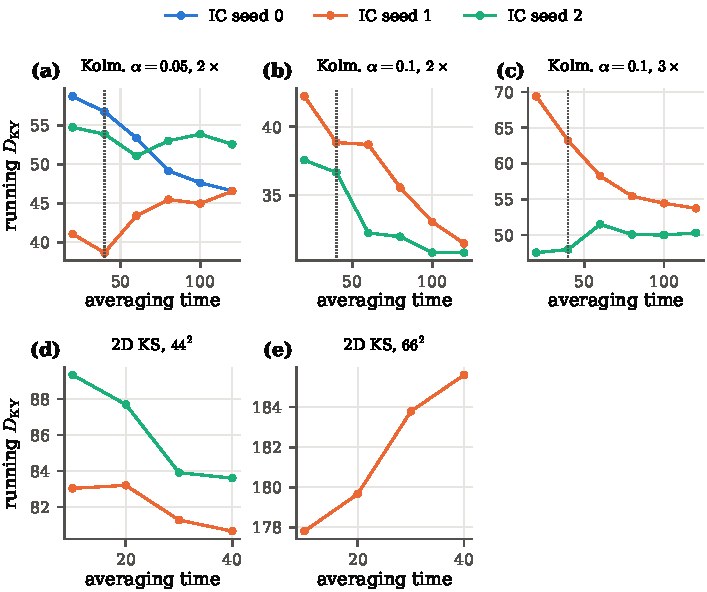
\includegraphics{figures/figC1_truth_convergence.pdf}
\caption{Running Kaplan--Yorke dimension of every truth run that
recorded it, one panel per system and size; colours distinguish initial
conditions within a panel. Kolmogorov runs (120 time units): the dotted
line marks the value a 40-unit run returns, which differs from the
120-unit value by $-17\%$ to $+23\%$ and in five of seven runs lies
above it (mean $+9\%$). 2D KS runs (40 time units): the running value still moves by
$3$--$5\%$, in both directions, over the last 20 time units
(Appendix~\ref{app:truth_ks2d}).}
\label{fig:truth_convergence}
\end{figure*}

\begin{table*}[htbp]
\caption{Running $\DKY$ of the 120-unit Kolmogorov truths at the
recorded averaging times, and the relative deviation of the 40-unit value
from the 120-unit value.}
\label{tab:running_dky}
\begin{ruledtabular}
\begin{tabular}{lccccccc}
run & 20 & 40 & 60 & 80 & 100 & 120 & dev.\ at 40 \\
\hline
\tabinput{tables/tabC_running_kolm}
\end{tabular}
\end{ruledtabular}
\end{table*}

Two observations bear on how the main results are read. First, five of
the seven 40-unit estimates are high, by $9\%$ on average, so the
remaining single-run 40-unit truths ($\alpha=0.1$, $1\times$;
$\alpha=0.05$, $3\times$; all sizes at $\alpha=0.025$) may be biased
upward; a model that matched the converged dimension exactly would then
appear to under-estimate it. This happened at $\alpha=0.1$, $3\times$:
the earlier 40-unit run gave $56.35$, the mean over it and the two
120-unit runs is $53.47$, and the selected model's error there fell from
$7.6\%$ to $2.6\%$. Second, the spread between initial
conditions does not shrink to zero with a longer window at the sizes we
use: at $\alpha=0.05$, $2\times$, the three converged values are $46.6$,
$46.6$ and $52.6$.

%----------------------------------------------------------------------
\subsection{Convergence and spread of the 2D KS truths}
\label{app:truth_ks2d}
%----------------------------------------------------------------------

The 2D KS truths average over 40 time units, about 7 Lyapunov times.
Three runs at $44^2$ give $81.8$, $80.7$ and $83.6$, and two at $66^2$ give
$192.5$ and $185.6$, a spread of $\pm1.8\%$ at both sizes.
Table~\ref{tab:running_ks2d} gives the running estimates of the runs that
recorded them: over the last 20 time units they still move by $3$--$5\%$,
in both directions. We therefore treat the 2D KS truths as uncertain at
the level of a few percent, comparable to the model errors of
Sec.~\ref{sec:canonical_results} and larger than the $2.5\%$ difference
between the mean densities at the two sizes.

\begin{table}[htbp]
\caption{Running $\DKY$ of the 2D KS truth runs that recorded it, at the
averaging times shown (time units after the warm-up), and the change over
the last 20 time units.}
\label{tab:running_ks2d}
\begin{ruledtabular}
\begin{tabular}{lccccc}
run & 10 & 20 & 30 & 40 & last 20 \\
\hline
\tabinput{tables/tabC_running_ks2d}
\end{tabular}
\end{ruledtabular}
\end{table}

%----------------------------------------------------------------------
\subsection{Model spectra and their precision}
\label{app:model_spectra}
%----------------------------------------------------------------------

Model spectra use all $\dlat$ tangent directions, a warm-up of 200
steps, 2000 steps and a QR factorization every 10 steps
(Sec.~\ref{sec:evaluation}). The tangent vectors are propagated in
single precision by forward-mode differentiation, and the QR is done in
double precision. To check that single precision does not bias the
result we repeated one model spectrum per system in double precision,
from three initial conditions each:

\begin{center}
\begin{tabular}{lccc}
\hline\hline
system & single & double & IC spread \\
\hline
1D KS, $L=100$ & $22.24$ & $22.24$ & $1.0\%$ \\
1D KS, $L=200$ & $44.64$ & $44.62$ & $0.7\%$ \\
2D KS, $44^2$ & $83.51$ & $83.76$ & $1.0\%$ \\
Kolm., $\alpha=0.05$, $1\times$ & $23.26$ & $22.75$ & $25\%$ \\
\hline\hline
\end{tabular}
\end{center}
The means over initial conditions agree to within $0.3\%$ in 1D and 2D
KS and to within $2.2\%$ in Kolmogorov flow, far inside the spread over
initial conditions. Single runs are a different matter: switching
precision changes the trajectory, and in Kolmogorov flow at the native
size it moves one run's $\DKY$ from $26.0$ to $22.0$. A model's own
finite-time estimate at that size is therefore uncertain by much more
than its precision, which is why we average over initial conditions and
do not interpret differences between single runs.

%----------------------------------------------------------------------
\subsection{Matched initial conditions at native size}
\label{app:matched_ics}
%----------------------------------------------------------------------

For Kolmogorov flow at $\alpha=0.05$, $1\times$, the truth script and the
model-evaluation script build the same solver configuration ($\nu$, $n$,
time step and spin-up, read from the training data's metadata by the
evaluation script and hard-coded in the truth script, and checked to
agree) and generate the initial condition by the same call with the same
seed. For a given seed the two initial conditions are therefore
identical, not merely drawn from the same distribution, and a model run
can be scored against the truth from its own initial condition. Matched
truths exist for seeds 0--2 ($22.46$, $20.52$, $21.63$).

%----------------------------------------------------------------------
\subsection{List of ground-truth runs}
\label{app:truth_list}
%----------------------------------------------------------------------

\begin{table}[htbp]
\caption{All ground-truth runs used in the paper. $n_+$: number of
positive exponents. 1D runs have no seed column: all use IC seed 0 and are
independent realizations in the sense of
Sec.~\ref{app:benettin}.}
\label{tab:truth_runs}
\scriptsize\renewcommand{\arraystretch}{0.85}
\begin{ruledtabular}
\begin{tabular}{llcccccc}
system & size & seed & $K$ & window & $\lambda_1$ & $n_+$ & $\DKY$ \\
\hline
\tabinput{tables/tabC_truth_runs}
\end{tabular}
\end{ruledtabular}
\end{table}

%======================================================================
\section{Full evaluation tables}
\label{app:tables}
%======================================================================

Tables~\ref{tab:evals_ks2d}--\ref{tab:evals_kolm0025} list every 2D model
evaluated in this work, including those that appear only in
Secs.~\ref{sec:results2d} and \ref{sec:failure}. Each entry gives the mean
$\DKY$ over initial conditions $\pm$ half the range, the number of
initial conditions, and the mean of the per-IC relative errors against
Table~\ref{tab:truth} (at Kolmogorov $\alpha=0.05$, $1\times$, each initial
condition against its matched-IC truth). Every individual evaluation,
with $\lambda_1$ and the number of positive exponents, is in
\texttt{artifacts/\allowbreak experiments/\allowbreak appendix\_D\_evaluations.csv}, generated with
these tables by \texttt{scripts/paper\_figures/tabD\_evaluations.py}. The
evaluation files themselves also store a truth value and an error; these
were computed against the truths available on the day of each
evaluation, several of which were later revised (Sec.~\ref{sec:truth_uncertainty}),
and are not used anywhere in this paper. The 1D evaluations are complete
in Table~\ref{tab:transfer1d}.

\para{The 12-channel models of Part~II.} The data assimilation experiments use a 12-channel sibling
of the 2D KS model, trained on noisy fields (Appendix~\ref{app:architecture}). Its $\DKY$ is $84.7$ at
$44^2$ and $188.5$ at $66^2$, against truths of $81.8$ and $192.5$ ($3.6\%$ and $2.1\%$); a 12-channel model
trained on clean fields gives $83.5$ and $190.4$ ($2.1\%$ and $1.1\%$), and the 6-channel model of Part~I
$1.7\%$ and $2.4\%$. Doubling the channels and training on noisy data leave the transfer of the dimension
within the spread of the truth runs (\texttt{artifacts/experiments/crop/p7c12*\_ks2d\_x*.json}; one
initial condition each).

Table~\ref{tab:spectra} gives, for the main-text models, the
reconstruction error of the autoencoder, the ratio of the decoded
rollout's standard deviation to the truth's, and the share of energy in
the lowest and highest wavenumber bands (1D and 2D KS: $|\bm k|<0.35$ and
$|\bm k|\ge1.4$; Kolmogorov flow: kinetic energy at $|\bm k|<1$ and
$|\bm k|\ge16$), from one initial condition and 1000 snapshots per size.

\begin{figure*}[htbp]
\centering
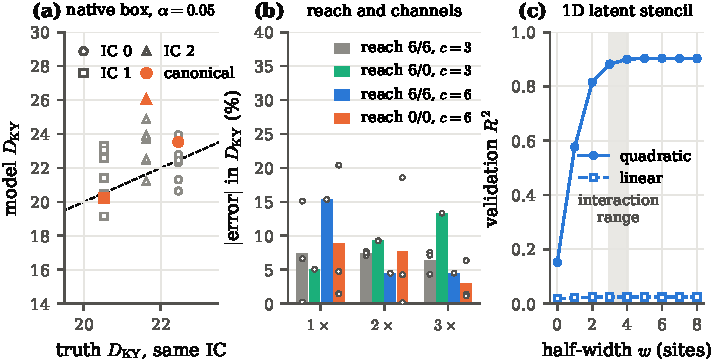
\includegraphics{figures/figC2_appendix_panels.pdf}
\caption{Supporting evidence. (a) Kolmogorov flow at $\alpha=0.05$, native
box: each model's $\DKY$ from one initial condition against the truth run
from the same initial condition (marker shape), for every model with
three native-size evaluations; filled: the canonical model; dashed: equality.
The truth varies by $\pm4.5\%$ across these initial conditions, single
models by $\pm1$--$12\%$. The models largely agree on the ordering, seven
of eight giving their largest value from IC~2, which the truth does not
share (its largest is from IC~0), so matching initial conditions removes
the truth's sampling noise but not the models'. (b) Reach and channel ablation at
$\alpha=0.05$, all trained on the same windows: encoder/decoder reach in
sites and number of channels; bars are means of $|$error$|$ over initial
conditions, dots individual initial conditions. (c) Interaction range of
the 1D latent dynamics: validation $R^2$ of one stencil, shared by all
sites, that predicts each site's one-step increment from the sites within
half-width $w$; the quadratic stencil saturates at $w=3$--$4$ sites
($19$--$25$ length units, shaded), the linear one explains almost
nothing (Sec.~\ref{sec:receptive}).}
\label{fig:appendix_panels}
\end{figure*}

\newcommand{\evalhead}[1]{model & description & #1 \\ \hline}
\newcommand{\evalnotes}{\par\footnotesize $^a$Trained on an $8\times8$-site
periodic box with the same architecture as the window-trained full-reach
models; the $\alpha=0.1$, $3\times$ value uses an unstandardized initial
condition, the only evaluation available. $^b$Narrow architecture
(encoder radius 1 over 2 layers, propagator window 1) trained on windows
of a $3\times$ periodic domain and evaluated on that domain.
$^\star$Main-text model.}

\begin{table*}[htbp]
\caption{2D KS: all evaluations. Columns: $44^2$, $66^2$, $88^2$ (no truth at $88^2$).}
\label{tab:evals_ks2d}
\widetabular{llccc}{\evalhead{$44^2$ & $66^2$ & $88^2$}
\tabinput{tables/tabD_ks2d}}
\evalnotes
\end{table*}

\begin{table*}[htbp]
\caption{Kolmogorov flow, $\alpha=0.1$: all evaluations (channel widths $1\times$, $2\times$, $3\times$).}
\label{tab:evals_kolm01}
\widetabular{llccc}{\evalhead{$1\times$ & $2\times$ & $3\times$}
\tabinput{tables/tabD_kolm01}}
\evalnotes
\end{table*}

\begin{table*}[htbp]
\caption{Kolmogorov flow, $\alpha=0.05$: all evaluations.}
\label{tab:evals_kolm005}
\widetabular{llccc}{\evalhead{$1\times$ & $2\times$ & $3\times$}
\tabinput{tables/tabD_kolm005}}
\evalnotes
\end{table*}

\begin{table*}[htbp]
\caption{Kolmogorov flow, $\alpha=0.025$: all evaluations.}
\label{tab:evals_kolm0025}
\widetabular{llccc}{\evalhead{$1\times$ & $2\times$ & $3\times$}
\tabinput{tables/tabD_kolm0025}}
\end{table*}

\begin{table}[htbp]
\caption{Reconstruction and decoded-rollout statistics of the main-text
models. ``recon.'': autoencoder error as a percentage of the field
variance; ``std'': decoded rollout standard deviation over the truth's;
the last two columns give the energy share (\%) in the lowest band for
truth / model rollout and in the highest band for truth /
reconstruction.}
\label{tab:spectra}
\begin{ruledtabular}\footnotesize
\begin{tabular}{llcccc}
system & size & recon. & std & low band & high band \\
\hline
\tabinput{tables/tabD_spectra}
\end{tabular}
\end{ruledtabular}
\end{table}

%======================================================================
\section{Data assimilation details}
\label{app:da}
%======================================================================

\subsection{Observation networks}
\label{app:da_networks}

Table~\ref{tab:da_networks} lists every configuration. The grid spacing
is that of the training data at every size, so a fixed stride is a fixed
physical spacing: two observations per site in 1D and four in 2D.
Observation errors are independent with standard deviation $0.1$ in
standardized units; $R=0.01\,I$.

\begin{table}[htbp]
\caption{Data assimilation configurations: grid, sites, latent dimension
$\dlat$, observation stride (grid points), spacing (length units) and
number of observations $m$.}
\label{tab:da_networks}
\begin{ruledtabular}
\begin{tabular}{llccccccccc}
system & size & grid & sites & $c$ & $\dlat$ & $K$ & offsets & stride & spacing & $m$ \\
\hline
\tabinput{tables/tabE_p2_networks}
\end{tabular}
\end{ruledtabular}
\end{table}

\subsection{Analysis schemes}
\label{app:da_filters}

Let $Z\in\R^{\Nens\times\dlat}$ be the forecast ensemble, $\bar z$ its mean,
$X=Z-\bar z$ the (optionally inflated) perturbations, $B=X^\top X/(\Nens-1)$,
$J$ the Jacobian of $h=\Hobs\circ\Dec$ at $\bar z$, and $\rho$ the
Gaspari--Cohn taper \citep{gaspari1999} of half-width $3$ sites, which
vanishes at site distances of 6 and more.

\para{Dense filter.} With perturbed observations
$y^{(e)}=y+\varepsilon^{(e)}$, $\varepsilon^{(e)}\sim\mathcal N(0,R)$,
\begin{equation}
\begin{aligned}
  z_a^{(e)} &= z^{(e)} + K\big(y^{(e)}-h(z^{(e)})\big),\\
  K &= (\rho\circ B)J^\top\big(J(\rho\circ B)J^\top+R\big)^{-1}.
\end{aligned}
\end{equation}
The innovation uses the nonlinear $h$; the gain uses $J$.

\para{Per-site filter.} For each site $s$, let $U_s$ be the observations
with $\rho(\dist(s,\mathrm{site}(i)))>0$, $N_s$ the sites that own them,
and $R_s=\mathrm{diag}(R_{ii}/\rho_i)_{i\in U_s}$. With $J_s$ the rows of $J$
in $U_s$ restricted to the columns of $N_s$ (exact by
Proposition~\ref{prop:blockdiag}), $B_{N_s}$ the sample covariance of the
sites in $N_s$ and $B_{s,N_s}$ that of site $s$ with them,
\begin{equation}
\begin{aligned}
  z_{a,s}^{(e)} &= z_s^{(e)} + K_s\big(y^{(e)}_{U_s}-h_{U_s}(z^{(e)})\big),\\
  K_s &= B_{s,N_s}J_s^\top\big(J_sB_{N_s}J_s^\top+R_s\big)^{-1}.
\end{aligned}
\end{equation}
The covariance $B_{N_s}$ is not tapered; localization acts only through
$R_s$ \citep{hunt2007}.

\para{Deterministic transform.} With the same $U_s$, $R_s$ and
$Y=X_{N_s}J_s^\top\in\R^{\Nens\times|U_s|}$,
\begin{equation}
\begin{aligned}
  \tilde P &= \big[(\Nens-1)I+YR_s^{-1}Y^\top\big]^{-1},\\
  \bar w &= \tilde P\,YR_s^{-1}\big(y-\overline{h(z)}\big)_{U_s},\\
  W &= \big[(\Nens-1)\tilde P\big]^{1/2},
\end{aligned}
\end{equation}
and site $s$'s analysis ensemble is $\bar z_s + (\bar w\mathbf 1^\top+W)^\top X_s$
\citep{hunt2007}. For a linear $h$ without localization it reproduces
the Kalman update computed with the ensemble covariance exactly (unit
test). At $44^2$ its skill is within $0.15$ of the perturbed-observation
version at every ensemble size (Table~\ref{tab:da_2d_ensemble}) and its
CPU time about $40\%$ lower.

\para{Particle flow filter.} The Gauss--Newton (``NAT'') variant of
\citet{huvanleeuwen2021} with the localized prior covariance $\rho\circ B$,
held fixed in pseudo-time, at most 100 pseudo-time steps.

\para{Sampling error correction.} The correction table of
\citet{anderson2012} is built by Monte Carlo for each ensemble size
(2000 trials per true correlation on a grid of 41 values in
$[-0.98,0.98]$, 100 bins). In \emph{matrix form} each sample correlation in
$B$ is replaced by its corrected value; the result need not be positive
semidefinite. The \emph{projected form} raises its eigenvalues to at
least $10^{-10}$ times the largest. The \emph{serial form} assimilates the
observations one at a time on the augmented state $[Z,h(Z)]$ and applies
the correction to each scalar regression coefficient,
$\beta_k=\mathrm{SEC}\big(\mathrm{corr}(x_k,\hat y_j)\big)\,\sigma_{x_k}\sigma_{\hat y_j}/(\sigma^2_{\hat y_j}+R_{jj})$.

\subsection{Cost of the observation Jacobian}
\label{app:da_jacobian}

Figure~\ref{fig:jacobian_timing} times the latent observation Jacobian at
every deployment size, with the observation network of the runs. The
coloured construction, $c=6$ forward-mode passes through the decoder,
gives the same matrix as dense reverse-mode differentiation to the last
digit (largest difference $0$ up to $132^2$), and its time grows slightly
more slowly than the latent dimension: $1.3$~ms at $44^2$ and $49$~ms at $440^2$.
Reverse mode needs one pass per observation and grows almost with the
square of the dimension, $52$ times slower at $132^2$; we did not run it
beyond that size.

\begin{figure}[htbp]
\centering
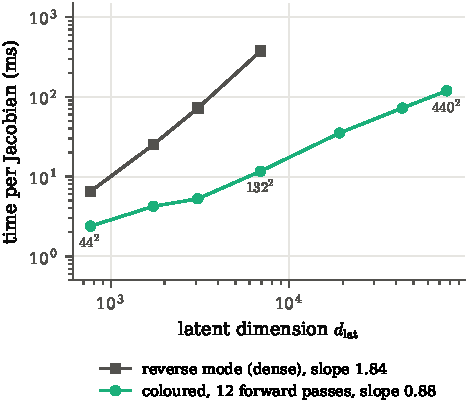
\includegraphics{figures/fig12_jacobian_timing.pdf}
\caption{Wall time per observation Jacobian against latent dimension,
2D KS, observation spacing $2.75$, four CPU threads, median of three: dense
reverse mode (one pass per observation) and the coloured construction
used by the per-site filter (six forward passes). The two agree exactly
where both were computed. Slopes are least-squares power-law fits.}
\label{fig:jacobian_timing}
\end{figure}

\subsection{Inflation, run-to-run spread and transients}
\label{app:da_tuning}

Multiplicative inflation of the forecast perturbations has little
effect (Table~\ref{tab:da_inflation}): the unlocalized filter is
unchanged to $1\%$, the per-site filter loses $4\%$ of its skill at
inflation $1.2$ and the dense localized filter $9\%$, and calibration moves
by at most $0.02$. With four observations per site and $R=0.01\,I$ the
analysis is dominated by the observations. All other runs use no
inflation.

A second seed, which changes the initial ensemble, the observation
noise and the model noise, changes the steady-state skill of the
per-site filter by $0.02$--$0.15$ at every size from $44^2$ to $330^2$ and that of the
unlocalized filter by $0.03$--$0.23$; differences below about $0.2$ in skill
are within run-to-run variation. The initial ensemble starts close to the
truth, so the analysis error first rises; it reaches its steady level
within $10$--$20$ cycles, after which its 10-cycle means vary by about
$\pm10\%$ at $44^2$ and $\pm3\%$ at $88^2$ and larger, the smaller domains averaging over
fewer independent regions. The per-cycle values of every run are stored
with its summary.

\begin{table}[htbp]
\caption{Steady-state skill (calibration) against multiplicative
inflation, 2D KS at $44^2$, 64 members.}
\label{tab:da_inflation}
\begin{ruledtabular}
\begin{tabular}{lcccc}
filter & 1.0 & 1.05 & 1.1 & 1.2 \\
\hline
\tabinput{tables/tabE_inflation}
\end{tabular}
\end{ruledtabular}
\end{table}

%======================================================================
\section{Reproducibility}
\label{app:reproducibility}
%======================================================================

\subsection{Code, results and provenance}

All results come from one Python package and its scripts. The package
(\texttt{ks\_latent}) contains the PDE solvers, the autoencoders and
propagators, the training loops including window training, the
Lyapunov analysis, and the filters; scripts run each experiment and write
a JSON file per run with its configuration, seeds and wall time. Every
table body and figure in this paper is produced by a script in
\texttt{scripts/paper\_figures/} that reads only these result files; each
figure is written with a sidecar file listing its inputs, the commit and a
time stamp. A decision log records every choice of truth, model and
convention and every correction made while writing. A number-provenance
check compares every decimal number in the text with the generated
tables and the result files and lists those it cannot match, each of
which has been checked by hand.
% TODO(G8): replace by the tagged release commit and archive DOI once the code is released; the
% results were produced from a working tree on top of commit 2cd9da0 with uncommitted changes.

\subsection{Numerics, devices and seeds}

The PDEs are integrated in double precision on the CPU with ETDRK4. The
networks are trained in single precision on the GPU of an Apple M5 Pro
(48~GB unified memory); training there is not bitwise reproducible, so
repeated trainings with one seed agree only statistically, and we report
separate training seeds where we have them. Lyapunov spectra propagate
tangent vectors in single precision and re-orthonormalize them in double
precision on the CPU (Appendix~\ref{app:model_spectra}); all filter linear
algebra is done in double precision on the CPU. Initial conditions are
indexed by seed (0, 1, 2) and spun up for 100--500 time units. PDE
trajectories from one seed are reproducible only for a fixed number of
FFT threads; runs that differ in thread count follow different
trajectories after a few Lyapunov times, and we use them as independent
realizations (Appendix~\ref{app:groundtruth}). The software environment
is Python 3.11.15, PyTorch 2.13.0, NumPy 1.26.4 and SciPy 1.17.1, fixed by
an exported environment file.

\subsection{Tests}

The properties the paper relies on are checked by unit tests, 132 of which
cover the claims below and pass in a few seconds:
\begin{itemize}
\item \emph{Solver:} the linear growth spectrum, the exponential
  time-differencing coefficients against high-precision evaluation, mean
  conservation, translation equivariance and fourth-order convergence.
\item \emph{Architecture:} exact translation equivariance of the 2D
  autoencoder along each axis (Proposition~\ref{prop:equivariance}); the
  gauge-anchored channel equals the patch average; the decoder Jacobian is
  exactly block-diagonal at zero reach (Proposition~\ref{prop:blockdiag}).
\item \emph{Window training:} a forced-halo rollout reproduces the
  interior of the same propagator run on the large periodic domain, in 1D
  and 2D, and a halo one site too narrow breaks the equality
  (Proposition~\ref{prop:halo}).
\item \emph{Lyapunov analysis:} the double-precision tangent path
  recovers the spectrum of a linear map to machine precision.
\item \emph{Observation Jacobian:} the coloured construction equals
  reverse-mode differentiation exactly, and the observation-to-site map
  is checked pixel by pixel; deployment grids keep the training spacing.
\item \emph{Filters:} with a linear observation operator and Gaussian
  prior, the particle flow filter, the dense and per-site ensemble Kalman
  filters and the serial filter converge to the Kalman posterior at large
  ensemble size; the deterministic per-site transform reproduces the
  Kalman update with the ensemble covariance exactly; sites beyond the
  taper support are left unchanged; the projected and serial forms of
  sampling error correction reduce to the plain filter for an identity
  correction.
\end{itemize}

\subsection{Compute}

All runs used one workstation. Typical costs: a 1D Lyapunov spectrum of
the PDE at $L=400$, 35~min; a 120-unit Kolmogorov truth at $3\times$, several
hours; a model spectrum at $3\times$ or $88^2$, about 7~min; training a 2D
propagator, 17~min to 2~h; a data assimilation run of 100 cycles,
$9$--$97$~s of wall time up to $88^2$ and $4$--$59$~min at $220^2$--$440^2$, with one or four
tilings (Table~\ref{tab:da_cost}).

\subsection{Part~II code}

The Part~II experiments are run by \texttt{scripts/exp\_h9\_tiled\_da.py} (the latent filter with
shifted tilings, forecasts and the robustness options), \texttt{scripts/exp\_i11\_pde\_letkf.py} (the
physics-based filter with wrong models, parameter estimation, bias correction and the hidden-field
truth), \texttt{scripts/exp\_i24\_phys\_emulator.py} (the learned model inside a physical-space
filter), \texttt{scripts/exp\_j16\_estimate\_pde\_model\_error.py} (offline one-cycle residuals),
\texttt{scripts/exp\_j17h\_fit.py} (best fits of the wrong-damping models) and
\texttt{scripts/exp\_j18b\_roundtrip.py} (the round-trip test). The noisy-data model is trained by
\texttt{scripts/train\_kolmogorov\_crop.py --data-noise 0.1}. The library modules are
\texttt{ks\_latent/da/letkf\_local.py} (per-site filter with RTPS), \texttt{letkf\_phys.py}
(physical-space filter, multi-field states), \texttt{param\_est.py} (parameter estimation),
\texttt{model\_error.py}, and in \texttt{ks\_latent/solver/} the wrong-model operators of
\texttt{ks2d.py}, the cached imperfect-model truths of \texttt{twin.py} and the hidden-field system of
\texttt{ks2d\_memory.py}, each with unit tests (the hidden-field solver against the exact solution of
its linearization; the joint parameter update against the ensemble Kalman regression). The queues
that ran every Part~II experiment are kept as \texttt{scripts/run\_*.sh}.


\section*{Open Research Section}
% TODO(G5): repository and DOI for code, trained models and the result files.
The code, trained models and result files that support the findings of this study, and the
scripts that produce every table and figure from them, are available from the corresponding
author upon reasonable request (Appendix~\ref{app:reproducibility}).

\section*{Conflict of Interest}
The authors have no conflicts to disclose.

\bibliography{refs}

\end{document}
